% ------------------------------------------------------------------------
% Title: Template for LMPS-themed thesis (main file)
% Authors:
%   - Flavien Loiseau (flavien.loiseau@ens-paris-saclay.fr),
%   - Alexandre Daby-Seesaram (alexandre.daby-seesaram@ens-paris-saclay.fr)
% Last update: 21/12/2023
% ------------------------------------------------------------------------

% !BIB TS-program = biber
% !BIB program = biber

\documentclass[12pt,a4paper,openright]{lmsbook}

%%% To remove
\usepackage{lipsum}

%%% Setup metadata
\hypersetup{
    pdfinfo={%
    Title={PostDoc Book},%
    Author={Alexandre Daby-Seesaram and Kateřina Škardová},%
    Subject={Working document on hybridising classical ROM and neural networks},%
    Creator={Alexandre Daby-Seesaram and Kateřina Škardová},%
    Keywords={HiDeNN, Neural networks, Tensor Decomposition, ROM},%    
    Org = {LMS École Polytechnique}},%
}
   
%%% Input files
% Bibliography
\addbibresource{biblio.bib}
% Notations
% \input{My}

%%% User packages
\usepackage{ToolsBook}
\usepackage{pdfpages} % To include pdf
% Remarks
\usepackage{amsthm}
\usepackage[most]{tcolorbox}
\tcbset{shield externalize} % Prevent tikz from externalizing tcolorbox
% Fontawesome for icons
\usepackage{fontawesome5}
% Cleverref for easier references
\usepackage[nameinlink,noabbrev,capitalise]{cleveref}
%%% User environments
% Remark
\newtheorem{myremark}{\color{accentcolor} {\footnotesize\reflectbox{\faComment[regular]}}~~Remark}[chapter]
\newtcolorbox{myremarkbox}{breakable,colback=accentcolor!5,boxrule=0pt,frame hidden,enhanced,borderline west={3pt}{0pt}{accentcolor}}
\newenvironment{remark}{%
    \begin{myremarkbox}
    \begin{myremark}
    }{%
    \end{myremark}
    \end{myremarkbox}
}
% Chapter summary
\newenvironment{chaptersummary}{%
    \section*{\faPenNib~~Summary of the Chapter}%
    \label{sec:summary_{\thechapter}}
    \stepcounter{section}
    \addcontentsline{toc}{section}{\protect\numberline{\thesection}Summary of the Chapter}
}{}

%%% User modifications
% Change default positioning arguments for floats (figures, tables, ...)
\makeatletter% because def contain @
    \def\fps@figure{hbpt!}
    \def\fps@table{hbpt!}
\makeatother

% Change itemize style 
\renewcommand\labelitemi{\color{accentcolor!80}\tiny{$\blacksquare$}}% bullet
\renewcommand\labelitemii{\color{accentcolor!60}\tiny{$\blacktriangleright$}}% --
\renewcommand\labelitemiii{\color{accentcolor!50}\tiny{$\bullet$}}% *

\begin{document}

%%% Frontmatter
\frontmatter
% Cover

\includepdf[pages=-]{chapters/Cover.pdf}    % Include the cover page
\clearpage{\thispagestyle{empty}\cleardoublepage}
\setcounter{page}{1}                        % Reset the page counter
% Frontmatter
\addcontentsline{toc}{chapter}{Front Matter}
\mtcaddchapter % Fix enabling minitoc to show correctly

% \chapter*{Acknowledgements}
% \addcontentsline{toc}{section}{Acknowledgements}

% % Table of contents
% \cleardoublepage
% \phantomsection%
\addcontentsline{toc}{section}{Contents}
\tableofcontents

% % List of tables
% \cleardoublepage
% \phantomsection%
% \addcontentsline{toc}{section}{\listtablename}
% \listoftables

% List of figures
\cleardoublepage
\phantomsection%
\addcontentsline{toc}{section}{\listfigurename}
\listoffigures

% % List of notations
% \cleardoublepage
% \phantomsection%
% \addcontentsline{toc}{section}{List of Symbols}  
% \listofnotations

\cleardoublepage

%%% Main matter
\mainmatter

% % Part I 
\part{Meetings}
% \chapter[The 18$^{\text{th}}$ of January 2024 - Requirements \& Initial understanding]{Initial progress report and discussion of future requirements}

{\color{accentcolor} \epigraph{How to get rich and famous}{M. G.}}

\begin{chapabstract}
    This is the review of the first meeting about our initial impressions and understanding of the Hierarchical Deep Neural Networks (HiDeNN).
\end{chapabstract}

\minitoc

\section{Progress report}
At the point of the meeting, we both have an implementation of a HiDeNN for solving the clamped 1D bar problem. Both of our implementations work when finding nodal coordinates onto a fixed mesh (i.e., solving the finite element problem by training the Neural Network and tuning the weight of the last hidden layer). However, there are still some issues when training the coordinates values of the mesh nodes. Indeed, the gradients are not correctly populated in deeper layers and the gradient of the loss w.r.t the coordinates only accounts for the operations occurring in the first layer. 

A manner to pass trainable arguments into forward functions and still populate their gradients for the downstream operations is yet to be found. A \href{https://discuss.pytorch.org/t/reusing-altered-parameters-in-more-than-one-layer/158106/2}{promising lead} was found by Katka at the end of the day, but it remains to be tested.

\Rq{The HiDeNN seems to be more a tensor optimisation using pytorch than a black box neural network.}

We have two different implementations. 
\begin{itemize}
    \item[\faCodeBranch] \textbf{Option a)} only relies on two ``global'' NN that are latter combined. 
    \item[\faCodeBranch] \textbf{Option b)} is more fragmented and is built on sub-neural networks that correspond to the elementary blocks described in \parencite{zhang_hierarchical_2021}.
\end{itemize}

\section{Required tools in the future}

For future application, several implementations are required. 
\begin{itemize}
    \item 1D bar elements 
    \begin{itemize}
        \item Linear
        \item Quadratic
    \end{itemize}
    \item 2D triangles
    \begin{itemize}
        \item Linear (T3)
        \item Quadratic (T6)
    \end{itemize}
    \item 2D quadrangles
    \begin{itemize}
        \item Linear
        \item Quadratic
    \end{itemize}
\end{itemize}

In order to use the Gauss quadrature, it is necessary to implement the reference element for each of these elements and to map the reference elements to the real elements. The reference elements are non-trainable blocks that are hard coded, and the mapping (relying on the actual nodal coordinates) is tuned through the training process. The mapping can remain linear even for quadratic shape functions for now.


\section{Spatial parameters}
An essential aspect for the future relies on non-uniform parameters across the considered geometry. Making patient-specific models also means adapting those parameter fields to each new patient. In order for the Neural Network (NN) to be usable for a new spatial distribution of parameters $\mu\left(x\right)$ (i.e., a new patient), the spatial distribution, somehow must be part of the input of the neural network (as opposed to solely inputting the value of the parameter at the coordinate we evaluate the NN).
% \subsection{Parameter field representation}
In order to account for the global aspect of the spatial distribution without relying on an enormous number of parameters, an idea is to project the parameter field onto a spatial basis of a reasonable size. The Parameter field would then read 
\begin{equation}
    \mu\left(x\right) = \sum_{i=1}^{n_p}\mu_i f_i\left(x\right), 
    \label{eq:Projection_parameterField}
\end{equation}
with $\left\{f_i\right\}_{i \ in \llbracket 1,n_p \rrbracket}$ a spatial basis composed of global functions. A naive (and inefficient) idea for the basis basis would be to use discontinuous Galerkin functions to span the parameter space. Later, a more suitable basis could instead be obtained using several training data (actual parameter fields). The patient-specific input values $\left\{\mu_i\right\}_{i \ in \llbracket 1,n_p \rrbracket}$ would then correspond to the coordinates of the projection of the new patient parameter field $\mu(x)$ onto the previously computed basis.

% \begin{figure}
%     \centering
%     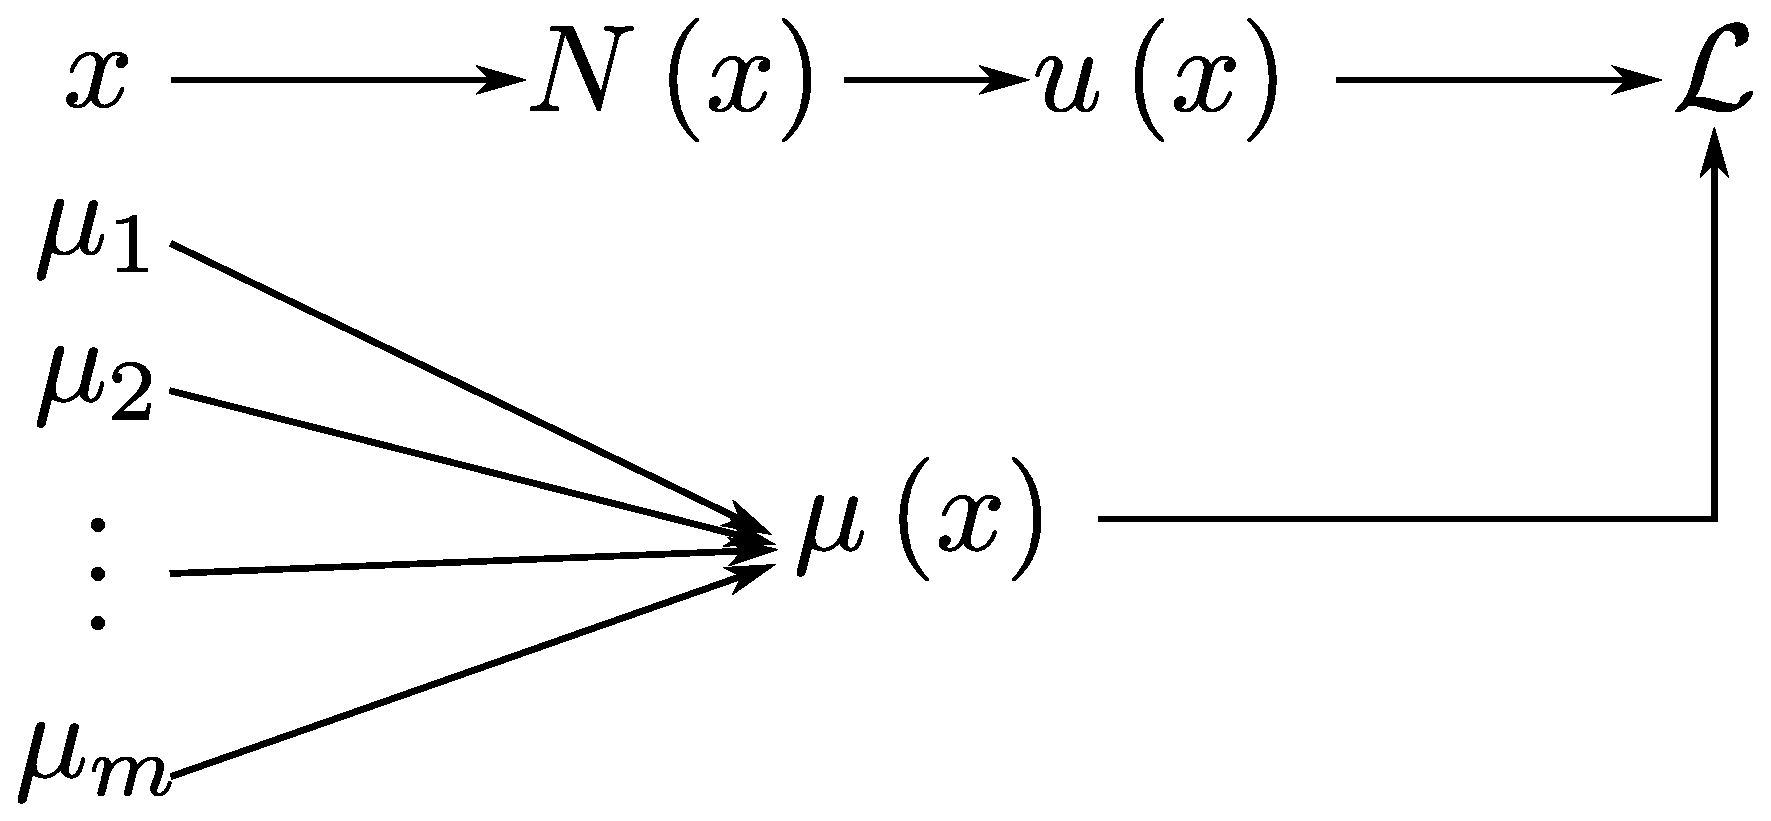
\includegraphics[width = 0.7\linewidth]{Figures/SpatialVariability_Parameters.eps}
%     \caption{Architecture of the HiDeNN parametrised with spatial parameter fields}
%     \label{SpatialVariability}
% \end{figure}

\begin{figure}[h]
    \centering
    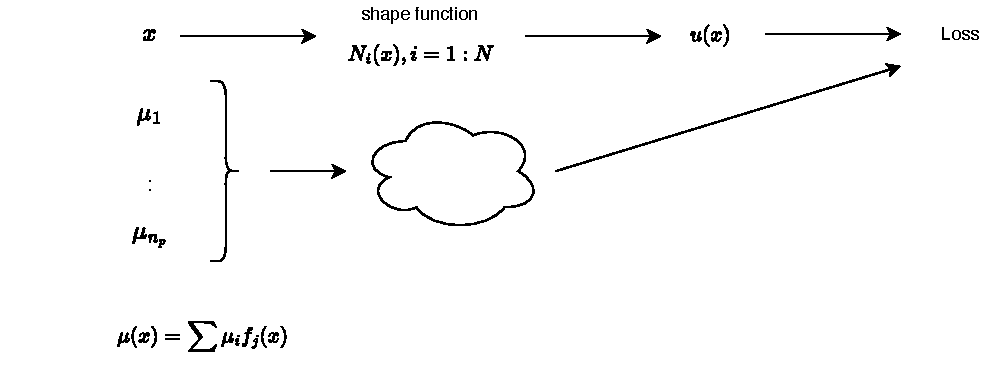
\includegraphics[width = 0.8\linewidth]{Figures/Diagram_1.pdf}
    \caption{Architecture of the HiDeNN parametrised with spatial parameter fields}
    \label{SpatialVariability}
\end{figure}

\section{Integral formulation of loss vs. Mixed formulation}

For the 1D test problem:
\begin{align*}
    \frac{\mathrm{d}}{\mathrm{d}x}\left( AE \frac{\mathrm{d}u}{\mathrm{d}x}\right) + b(x) = 0 \quad x\in [0,10]
\end{align*}
we use (i) integral loss function approach, (ii) mixed formulation approach. 

In (i) we perform forward pass of NN to get $u(x)$ for all training points $x$, then evaluate loss, compute gradient and update NN weights. To evaluate the loss, we use $\frac{\mathrm{d}u}{\mathrm{d}x}$ obtained by autograd -- linear shape functions are sufficient.

In (ii), we define two NNs: one for prediction of $u(x)$ and one for prediction of $s(x) = E\frac{\mathrm{d}u}{\mathrm{d}x}$. Loss function consists of two terms:
\begin{align*}
    \mathrm{Loss}(x) = \| \frac{\mathrm{d}}{\mathrm{d}x}\left( As(x)\right) + b(x)\|^2 + \| s(x) - E\frac{\mathrm{d}u}{\mathrm{d}x}\|^2
\end{align*}
The training points are processed individually or in batches  -- weights are be updated after evaluation of each points / batch. We use NN with quadratic shape functions for predictions of $u$ and NN with linear shape function for predictions of $s$.
\begin{figure}[h!]
    \centering
    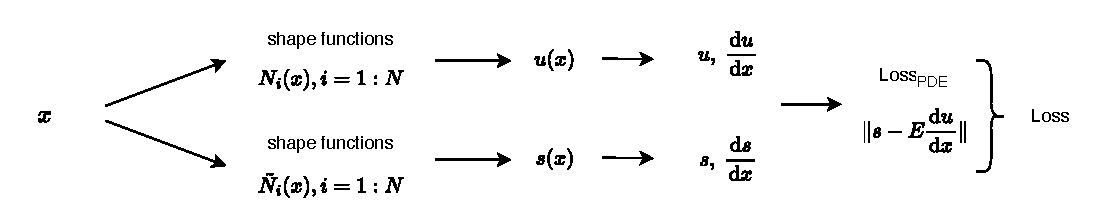
\includegraphics[width = 0.8\linewidth]{Figures/Diagram_2.pdf}
    \caption{The two NNs used for the mixed formulation.}
\end{figure}

% \Ccl{The HiDeNN framework seems to offer a nice way of building a ROM in a parametric context. }

% \Persp{See how to use the Tensor Decomposition}
% \chapter[The 25$^{\text{th}}$ of January 2024 - First results \& comments about HiDeNN]{First results \& comments about HiDeNN}

\begin{chapabstract}
    This chapter gives first results and comments about HiDeNNs
\end{chapabstract}

\minitoc

\section{Loss function}
Just like with regular PINNs, the loss function constrains the neural network to be physically consistent.
\subsection{Physical term}
 The first possibility is to use the potential energy of the system 
\begin{equation}
    \mathcal{L} = J\left(\vect{u}\right) = \frac{1}{2}\int_{\Omega} AE\left(\frac{\mathrm{d}\vect{u}}{\mathrm{d}x}\right)^2\mathrm{d}x - \int_{\Omega} \vect{u} \cdot \vect{b} \mathrm{d}x
\end{equation}
as a loss function as the solution minimises the potential energy. A disadvantage of doing so is that there are no easily chosen criteria to stop the training as the loss function drops below zero without any prior knowledge of the inferior bound of such a function as shown in \cref{fig:Loss_zoom}.

\begin{figure}
    \centering
    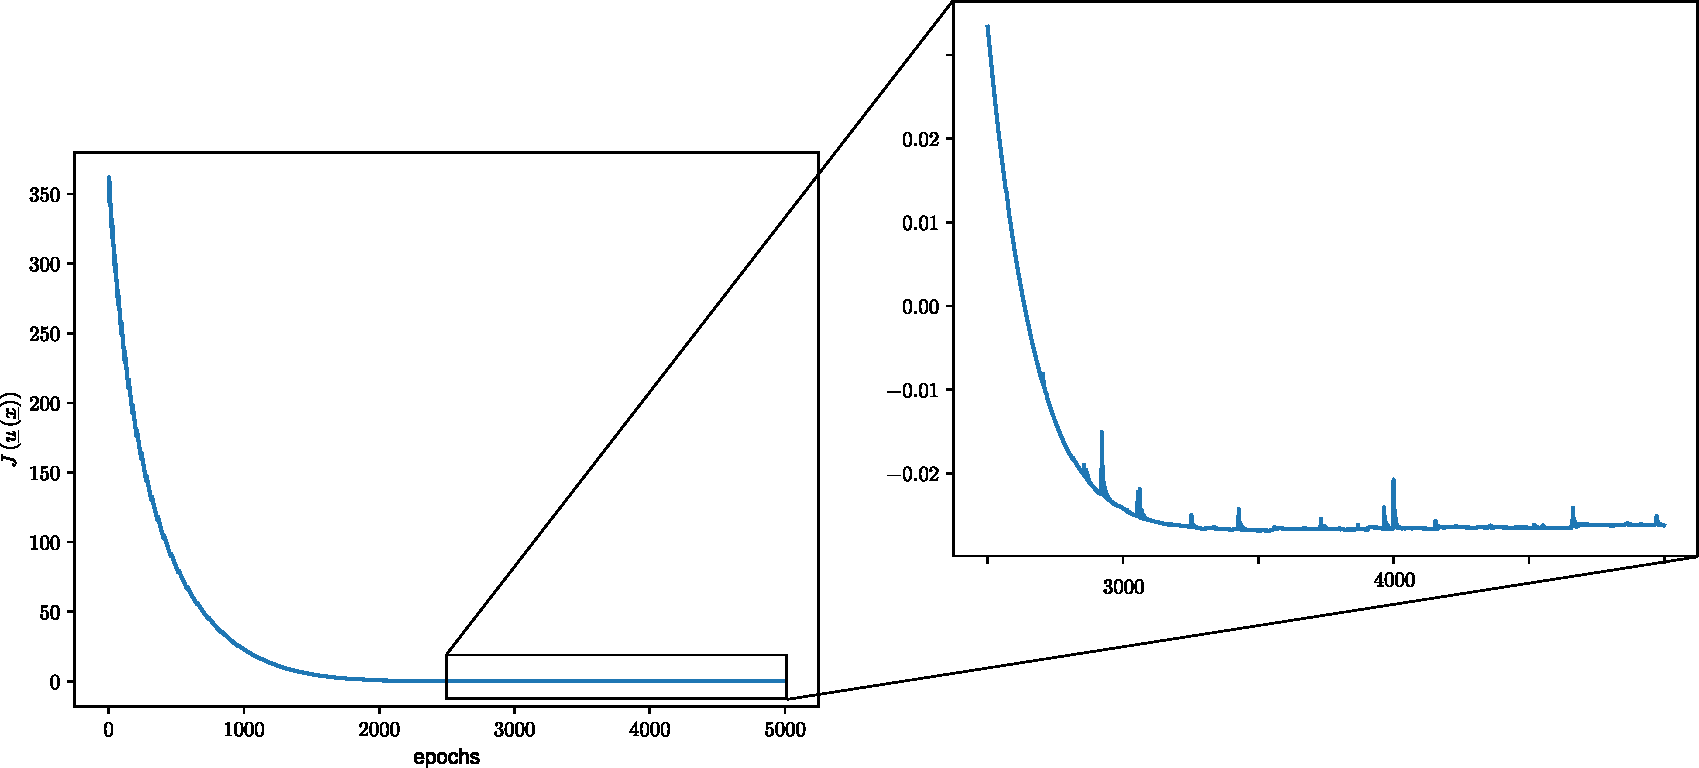
\includegraphics[width=\linewidth]{Figures/Loss_with_zoom.pdf}
    \caption{Potential energy $J\left(\vect{u}\right)$}
    \label{fig:Loss_zoom}
\end{figure}

A comparison of the information given by the decrease of the loss and the decrease of the $\ell^2$-error is given in \cref{fig:L2_vs_PE}, which highlights that the global behaviour of decay of both indicators agrees reasonably well.

\begin{figure}
    \centering
    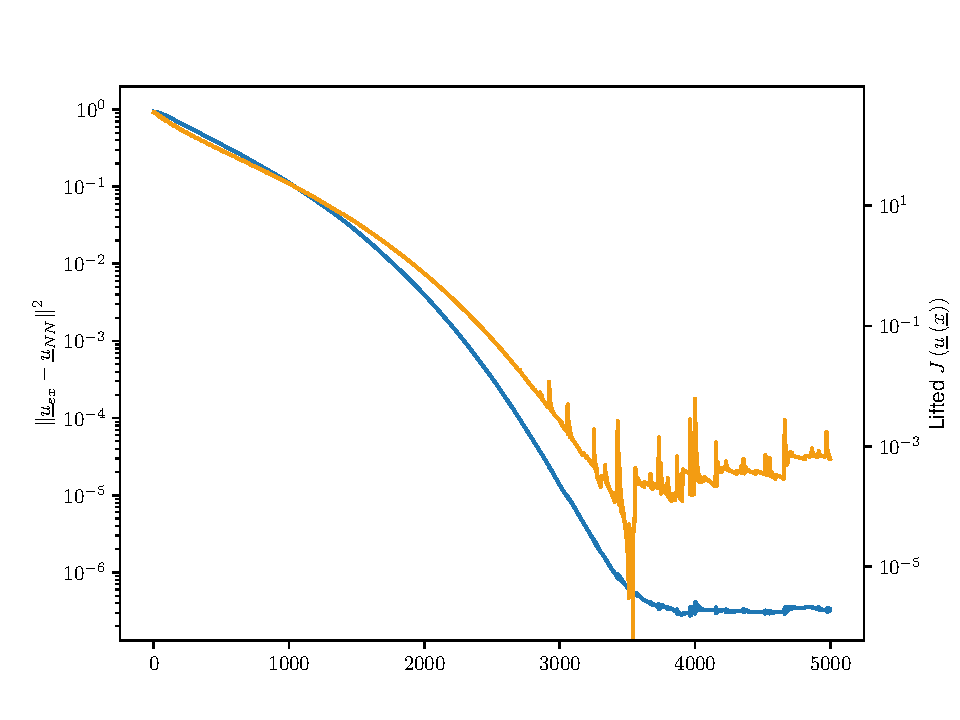
\includegraphics[width=0.7\linewidth]{Figures/Loss_Comaprison.pdf}
    \caption{Lifted $\mathcal{L}$ compared to  $\ell^2$-error}
    \label{fig:L2_vs_PE}
\end{figure}

\subsection{Regularisation term}

In order to avoid having distorted or even inside-out elements, a regularisation term is proposed so that the loss reads

\begin{equation}
    \mathcal{L} \triangleq\underbrace{ \mathcal{J\left(\vect{u}\right)} }_{\text{Physical loss}} + ~\alpha \underbrace{\left(\frac{\max J\left(x_i\right)}{\min J\left(x_i\right)} - 1\right)}_{\text{Mesh regularisation}},
\end{equation}
where 
\begin{equation}
    \left(\frac{\max J\left(x_i\right)}{\min J\left(x_i\right)} - 1\right) \ge 0
\end{equation}
and $\alpha$ is a weight for the regularisation term.

\Rqs{This implies using additional hyper-parameters whose choice needs to be automated}{This tends to force the mesh to be uniform, so it might not be optimal in the future when we want localised refinements.}
\section{First results with $n_p=23$ \& $n_p=10$}
\subsection{Without regularisation}
The HiDeNN set up with the ADAM optimiser and allowing both the nodes coordinates and nodal values to be trained leads to the following results given in \cref{fig:FirstSol}. Here no regularisation is used, the nodes are just forbidden to cross one another.
\begin{figure}
    \begin{subfigure}{0.5\linewidth}
        \centering
        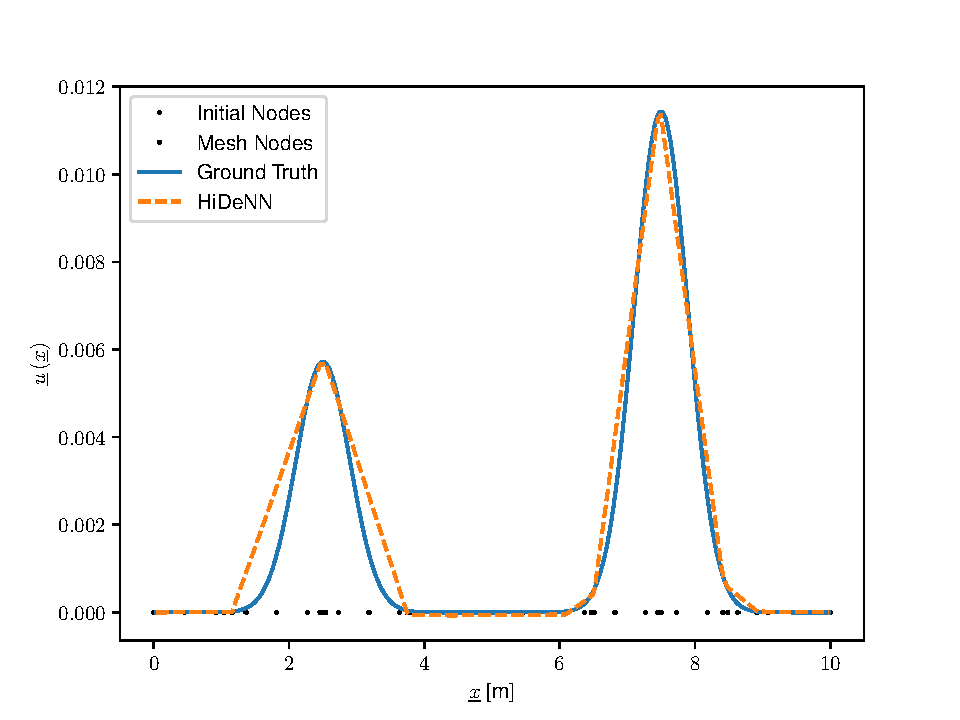
\includegraphics[width=\linewidth]{Figures/Solution_displacement.pdf}
        \caption{Displacement solution}
    \end{subfigure}
    \begin{subfigure}{0.5\linewidth}
        \centering
        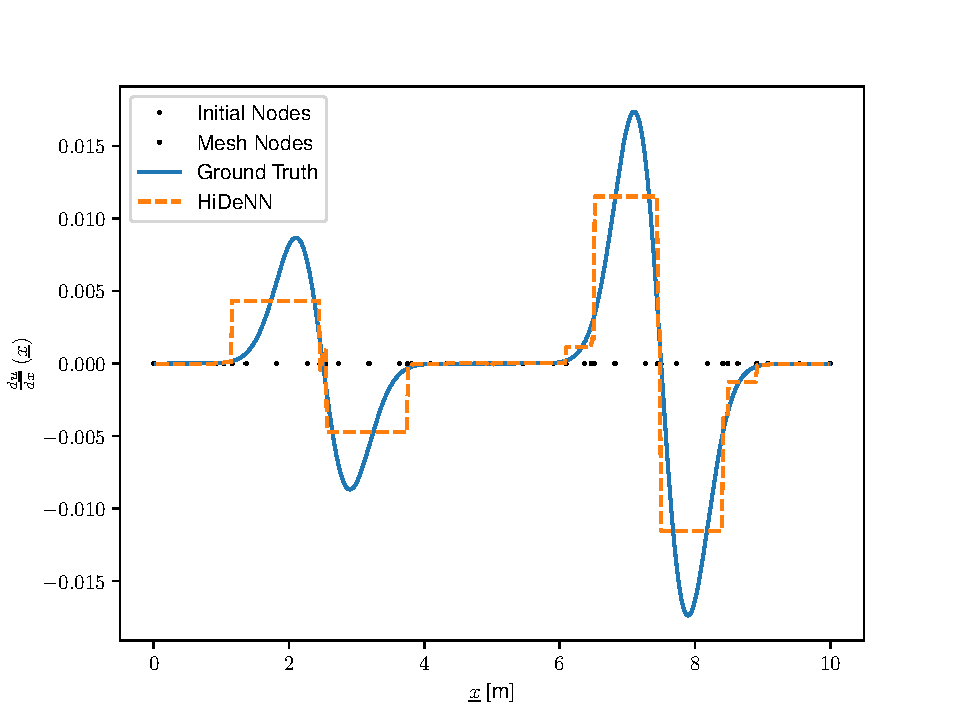
\includegraphics[width=\linewidth]{Figures/Solution_gradients.pdf}
        \caption{Displacement's first derivative}
    \end{subfigure}
    \caption{Comparison of NN's solutions with analytical solutions}
    \label{fig:FirstSol}
\end{figure}
The coordinates' optimisation process during training can be monitored by looking at their trajectories as shown in \cref{fig:Traj}.
\begin{figure}
    \centering
    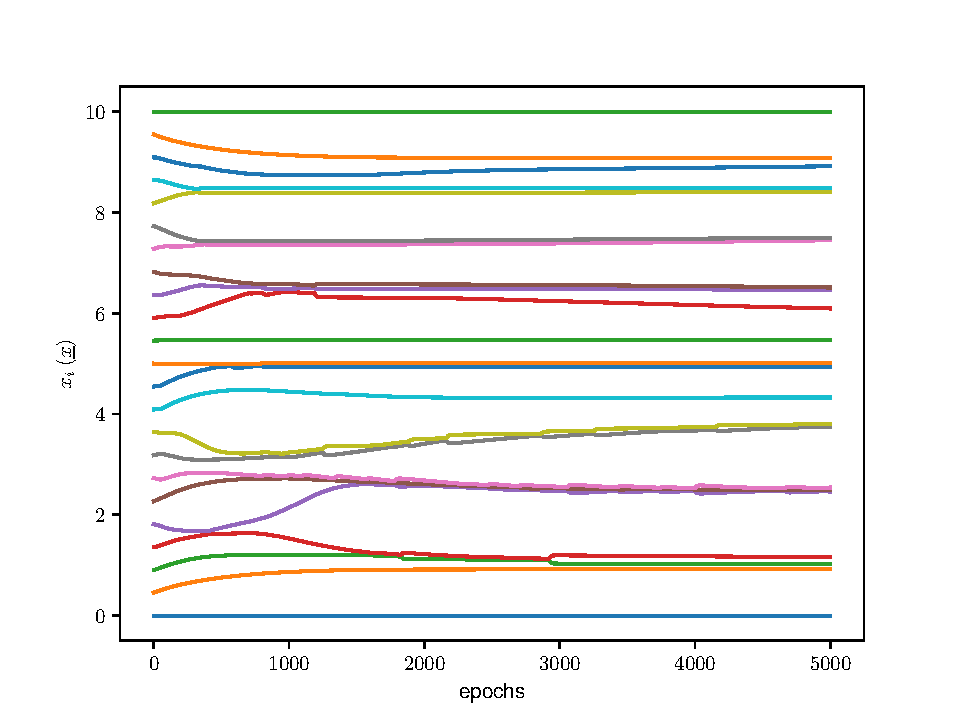
\includegraphics[width=0.5\linewidth]{Figures/Trajectories.pdf}
    \caption{Trajectories of the nodal coordinates without regularisation}
    \label{fig:Traj}
\end{figure}

\Rq{The nodes seem to be competing for the same position.}


\subsection{With regularisation (\& in double precision [\code{float64}])}

The comparison of the solution with the analytical solution is given in \cref{fig:FirstSol_regul}, and the loss and trajectories are given in \cref{fig:Loss_traj_regul}.
\begin{figure}
    \begin{subfigure}{0.5\linewidth}
        \centering
        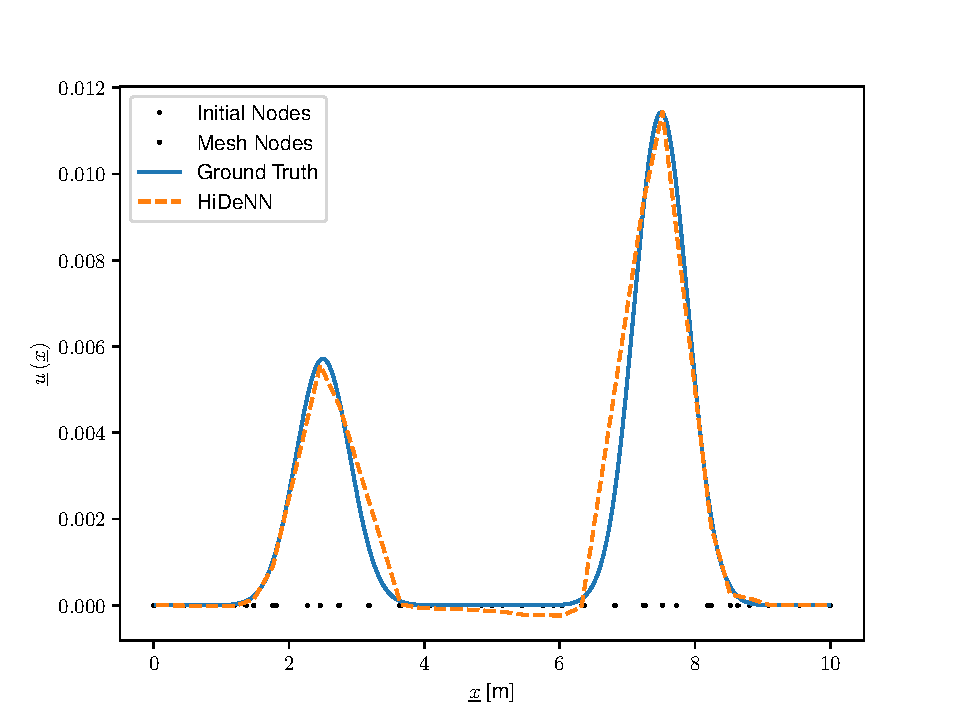
\includegraphics[width=\linewidth]{Figures/Solution_displacement_Regul64.pdf}
        \caption{Displacement solution}
    \end{subfigure}
    \begin{subfigure}{0.5\linewidth}
        \centering
        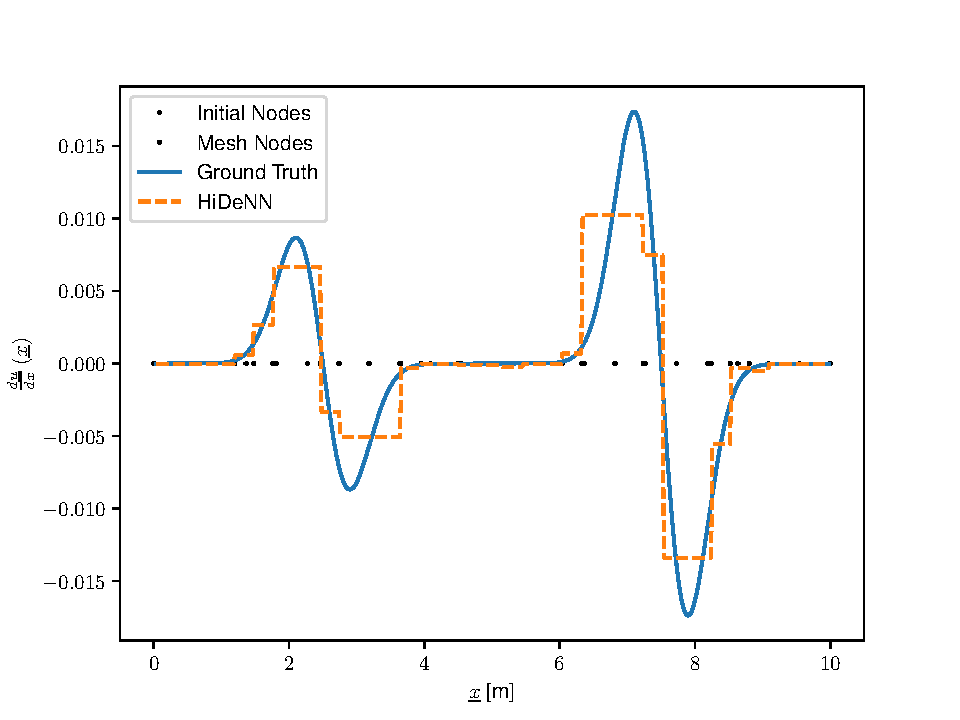
\includegraphics[width=\linewidth]{Figures/Solution_gradients_Regul64.pdf}
        \caption{Displacement's first derivative}
    \end{subfigure}
    \caption{Comparison of regularised NN's solutions with analytical solutions}
    \label{fig:FirstSol_regul}
\end{figure}
\begin{figure}
    \begin{subfigure}{0.5\linewidth}
        \centering
        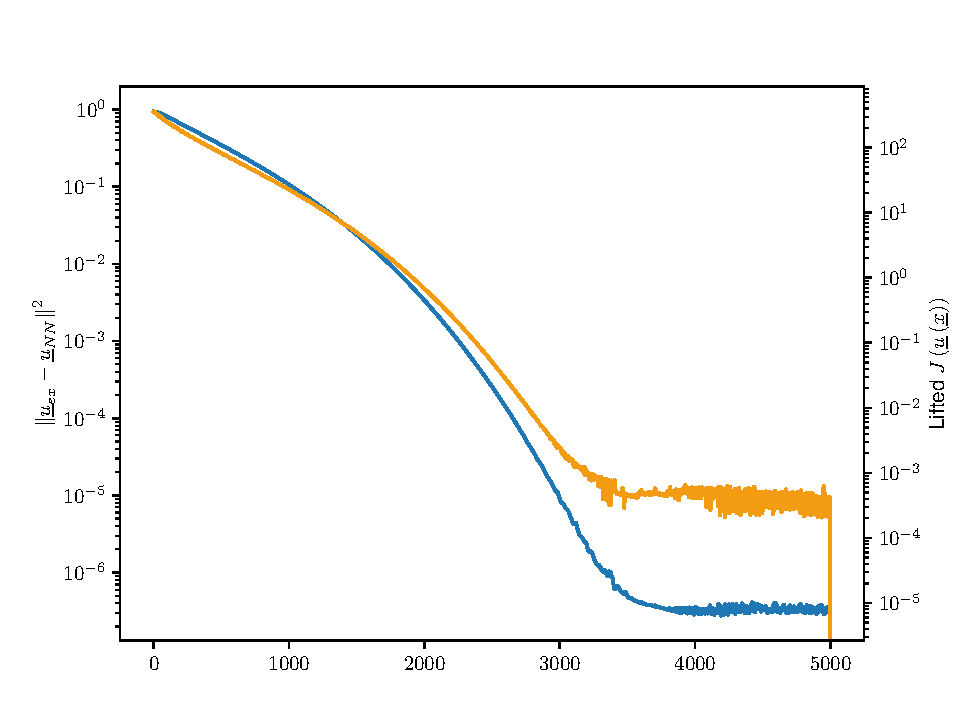
\includegraphics[width=\linewidth]{Figures/Loss_Comaprison_Regul64.pdf}
        \caption{Loss and $\ell^2$-error}
    \end{subfigure}
    \begin{subfigure}{0.5\linewidth}
        \centering
        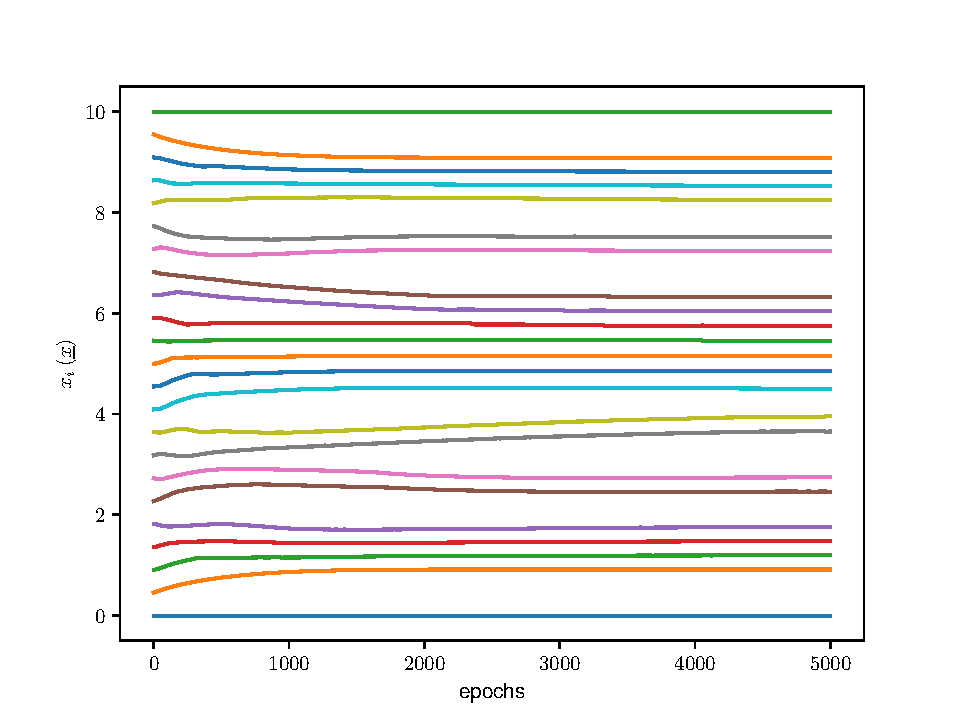
\includegraphics[width=\linewidth]{Figures/Trajectories_Regul64.pdf}
        \caption{Trajectories of the coordinates}
    \end{subfigure}
    \caption{Evolution of the loss and the $\ell^2$-error and evolution of the nodal coordinates with regularisation}
    \label{fig:Loss_traj_regul}
\end{figure}

\subsection{Influence of the mesh adaptivity}
\paragraph{$n_p=23$}
For $n_p=23$ the mesh adaptivity does not improve the solution

\begin{figure}
    \begin{subfigure}{0.3\linewidth}
        \centering
        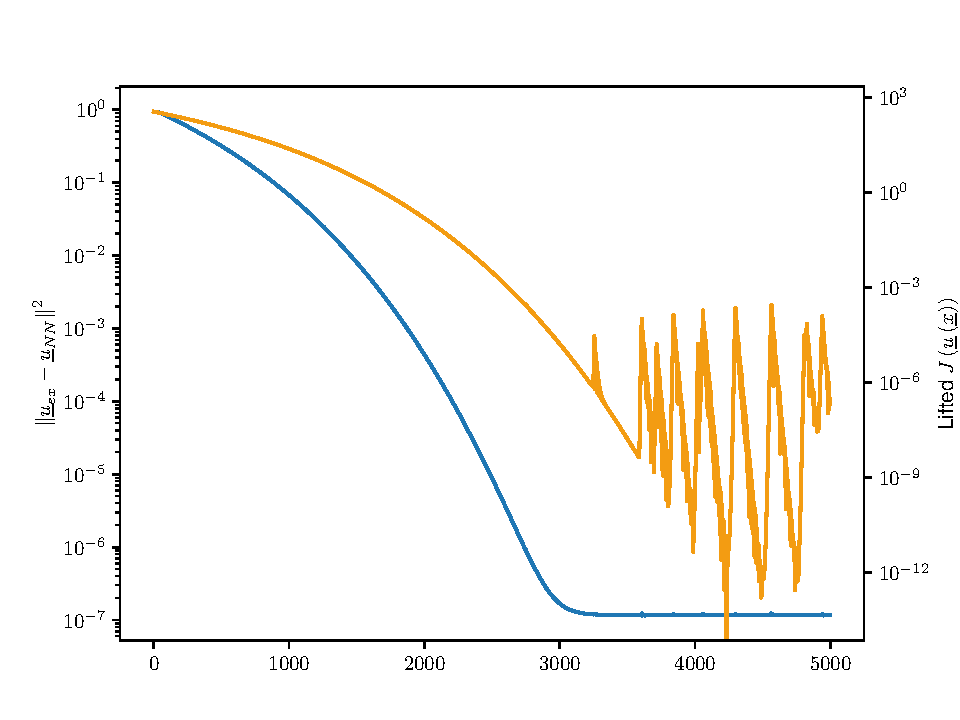
\includegraphics[width=\linewidth]{Figures/Loss_Comaprison_Frozen.pdf}
        \caption{Evolution of the loss}
    \end{subfigure}
    \begin{subfigure}{0.3\linewidth}
        \centering
        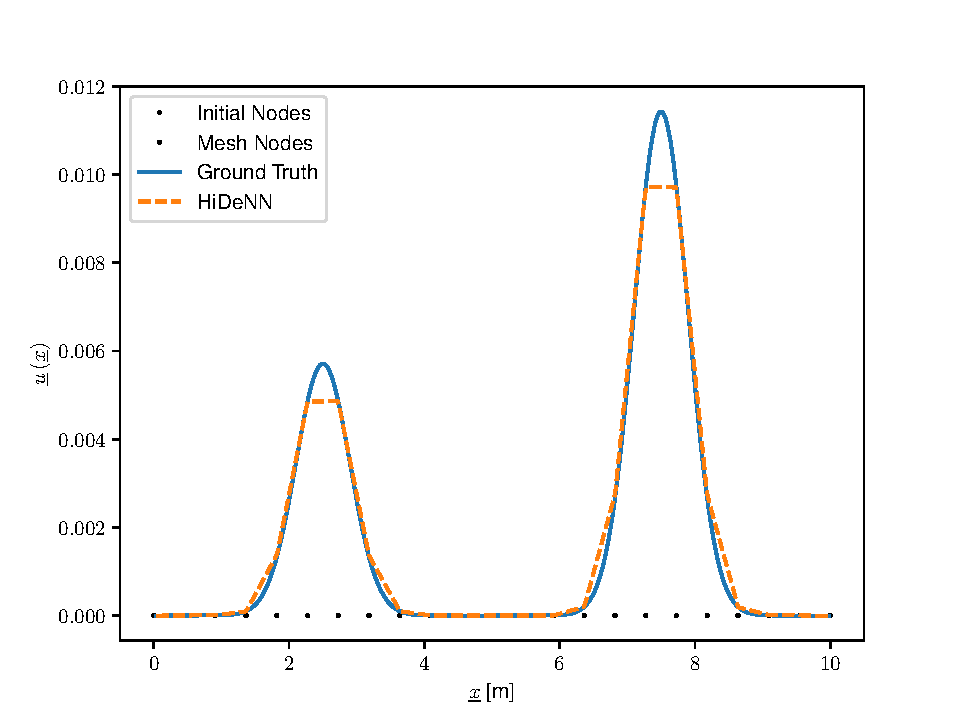
\includegraphics[width=\linewidth]{Figures/Solution_displacement_Frozen.pdf}
        \caption{Displacement}
    \end{subfigure}
    \begin{subfigure}{0.3\linewidth}
        \centering
        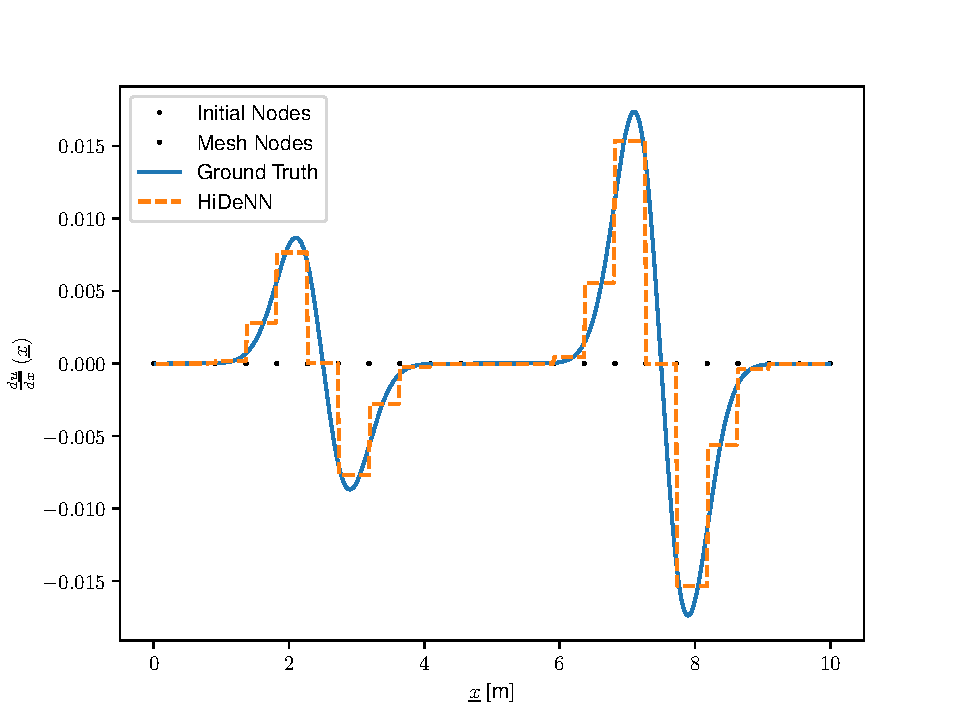
\includegraphics[width=\linewidth]{Figures/Solution_gradients_Frozen.pdf}
        \caption{Gradient}
    \end{subfigure}
    \caption{Fixed mesh - $n_p=23$}
    \label{fig:Fixed Mesh23}
\end{figure}

\begin{figure}
    \begin{subfigure}{0.3\linewidth}
        \centering
        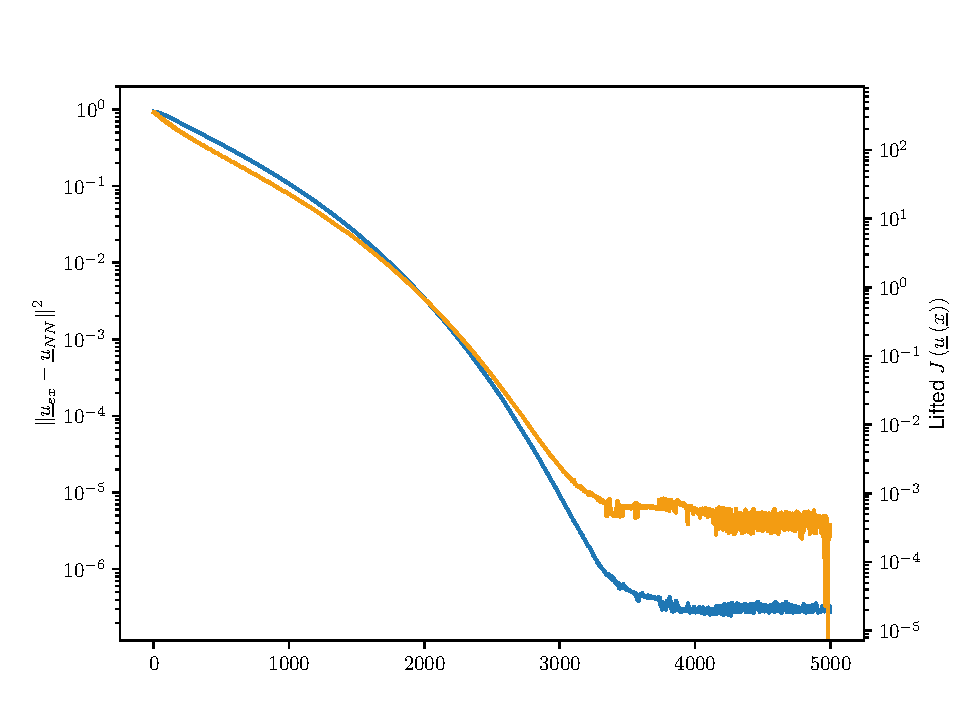
\includegraphics[width=\linewidth]{Figures/Loss_Comaprison_Regul32.pdf}
        \caption{Evolution of the loss}
    \end{subfigure}
    \begin{subfigure}{0.3\linewidth}
        \centering
        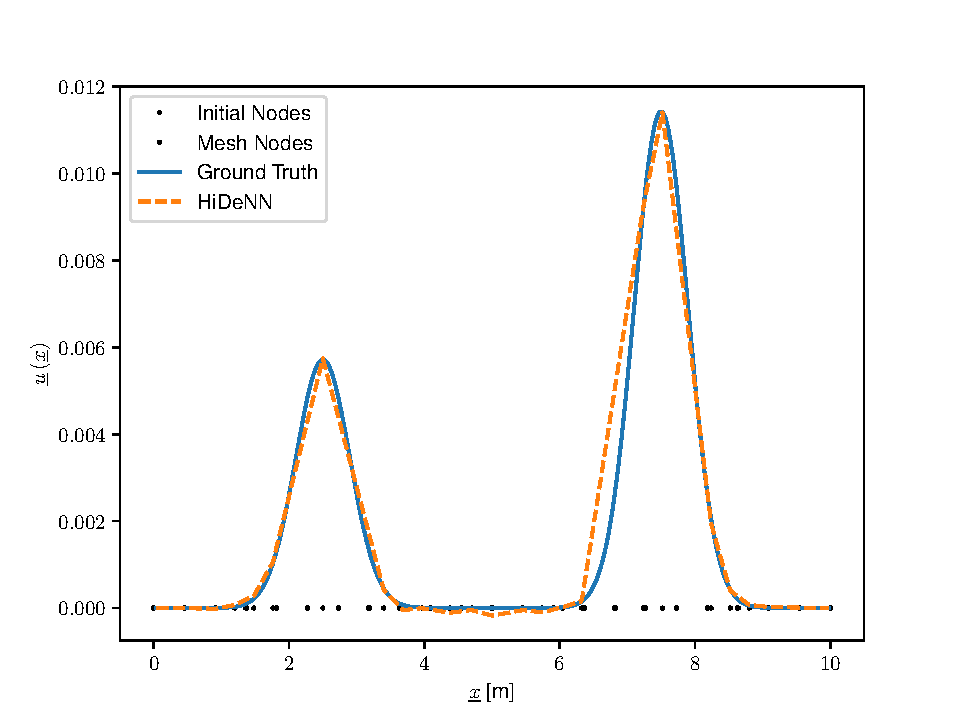
\includegraphics[width=\linewidth]{Figures/Solution_displacement_Regul32.pdf}
        \caption{Displacement}
    \end{subfigure}
    \begin{subfigure}{0.3\linewidth}
        \centering
        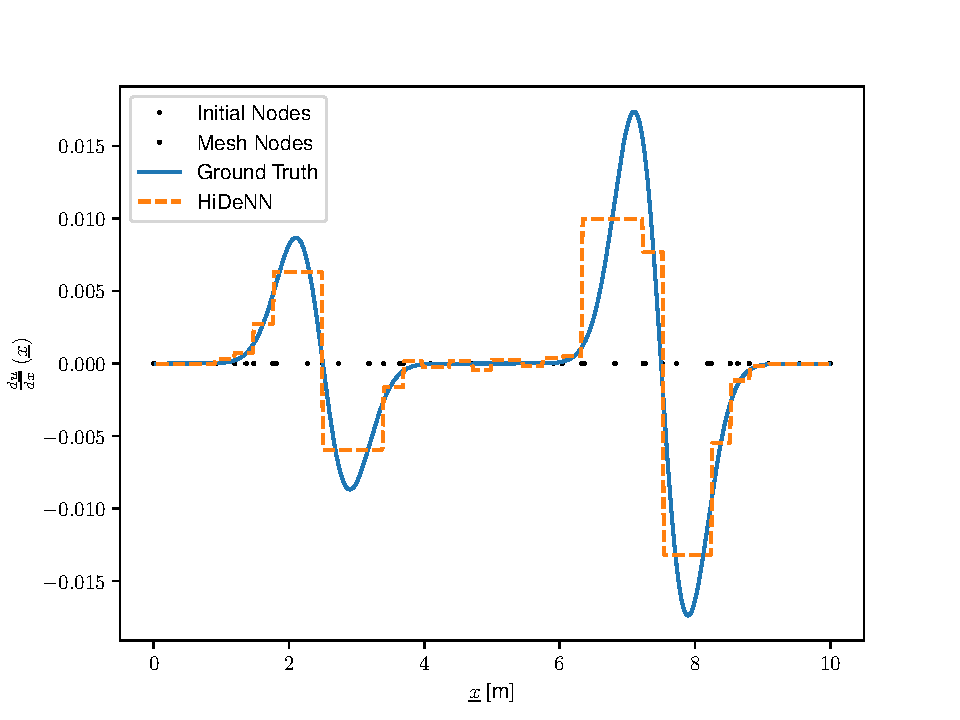
\includegraphics[width=\linewidth]{Figures/Solution_gradients_Regul32.pdf}
        \caption{Gradient}
    \end{subfigure}
    \caption{Free mesh float 32 - $n_p=23$}
    \label{fig:Fixed_Mesh23Float32}
\end{figure}

\begin{figure}
    \begin{subfigure}{0.3\linewidth}
        \centering
        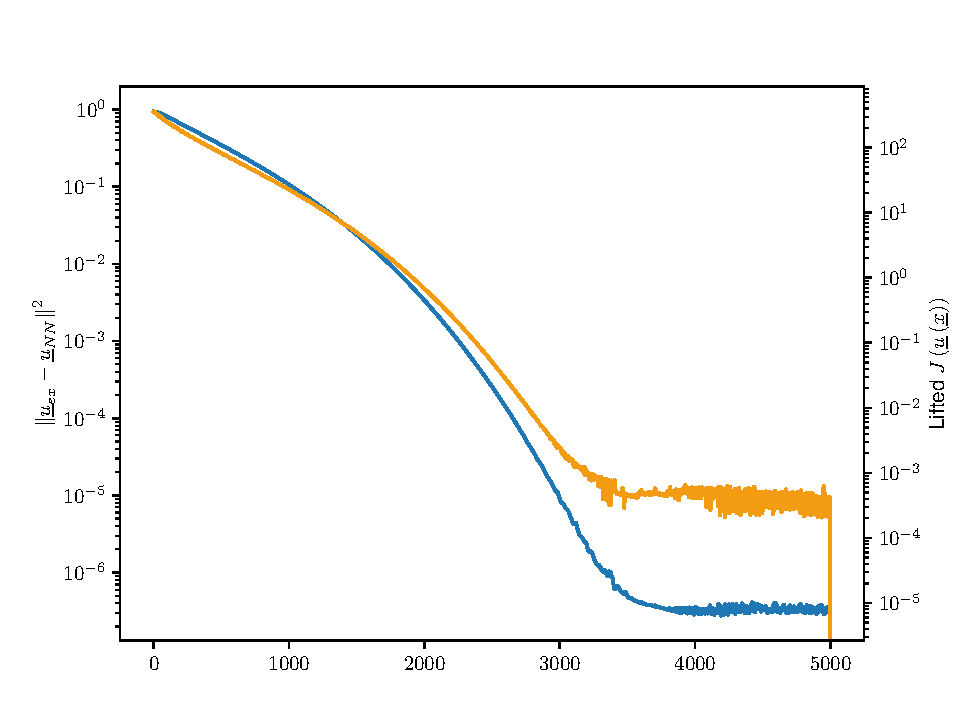
\includegraphics[width=\linewidth]{Figures/Loss_Comaprison_Regul64.pdf}
        \caption{Evolution of the loss}
    \end{subfigure}
    \begin{subfigure}{0.3\linewidth}
        \centering
        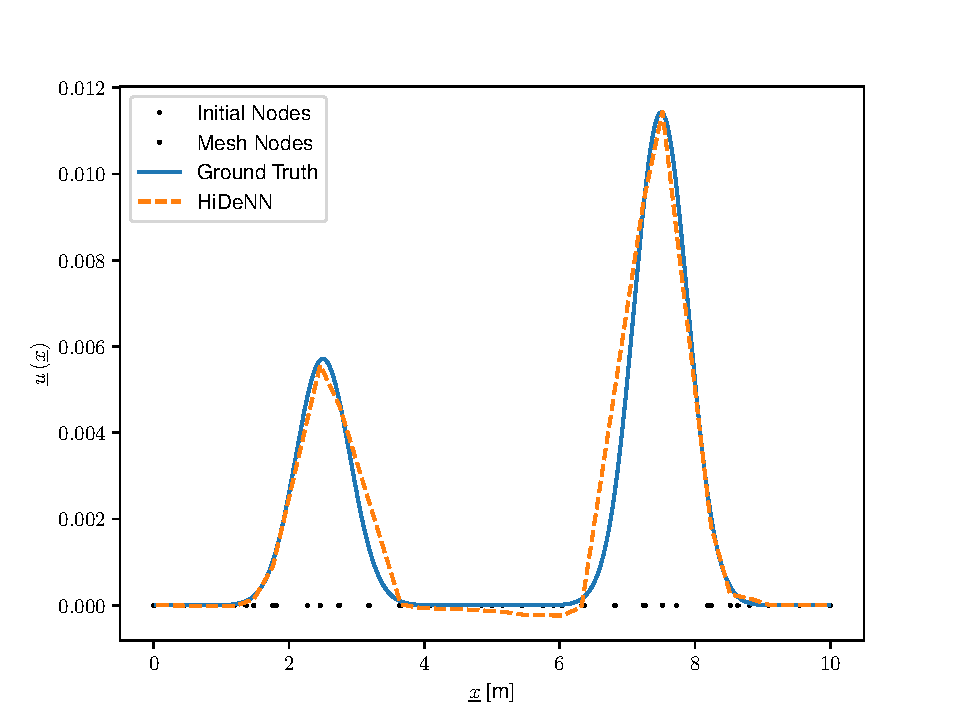
\includegraphics[width=\linewidth]{Figures/Solution_displacement_Regul64.pdf}
        \caption{Displacement}
    \end{subfigure}
    \begin{subfigure}{0.3\linewidth}
        \centering
        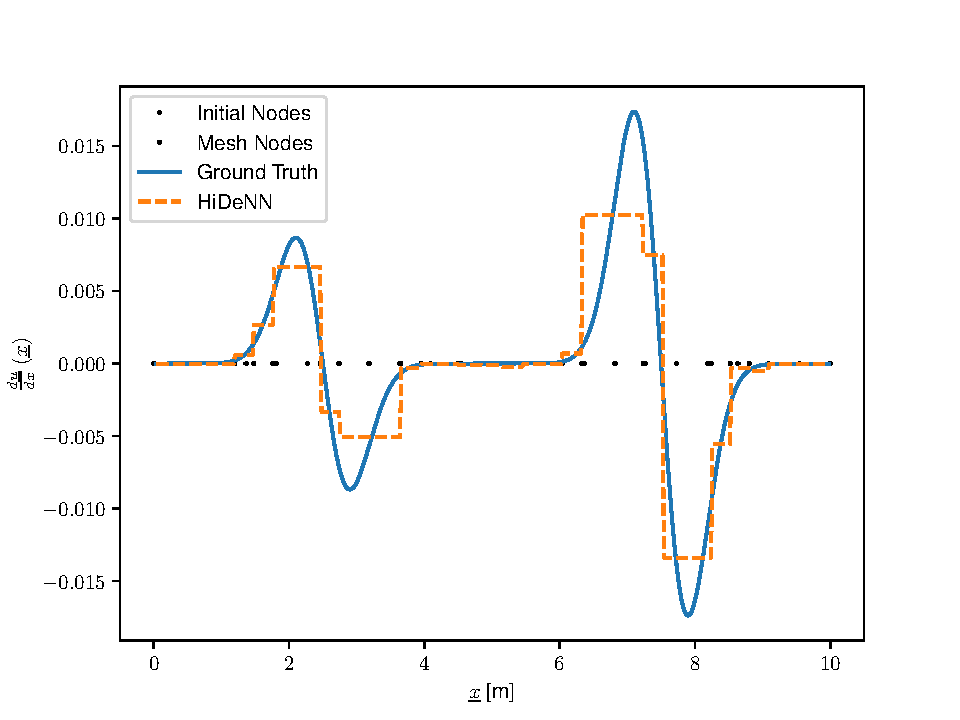
\includegraphics[width=\linewidth]{Figures/Solution_gradients_Regul64.pdf}
        \caption{Gradient}
    \end{subfigure}
    \caption{Free mesh float 64 - $n_p=23$}
    \label{fig:Fixed_Mesh23Float64}
\end{figure}


\paragraph{$n_p=10$}

For $n_p=10$ the mesh adaptivity improves the solution.


\begin{figure}
    \begin{subfigure}{0.3\linewidth}
        \centering
        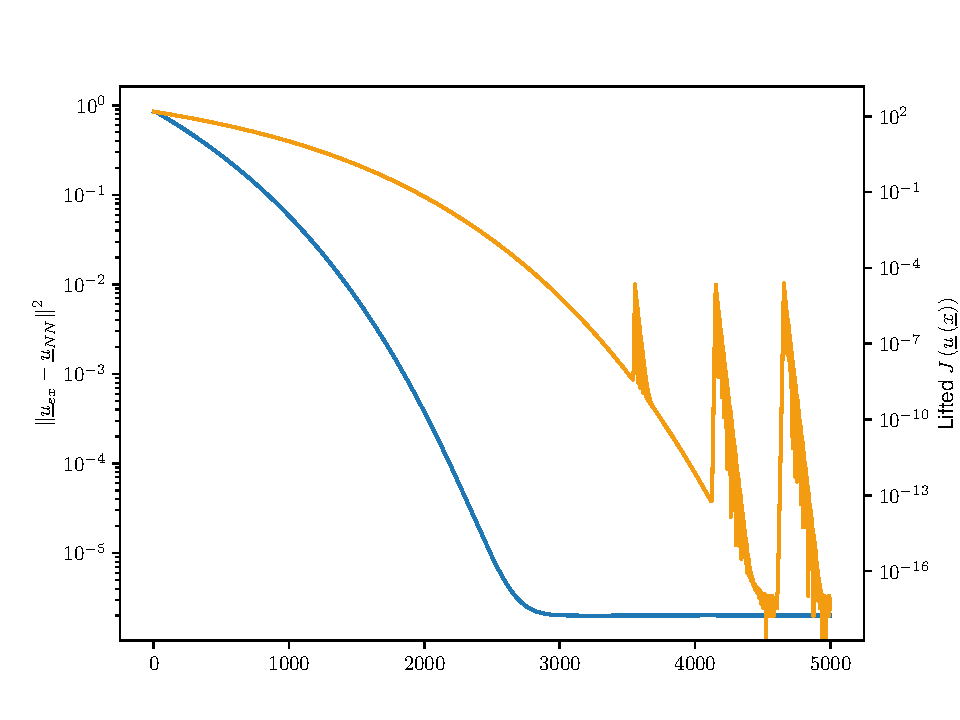
\includegraphics[width=\linewidth]{Figures/Loss_Comaprison_10_Frozen.pdf}
        \caption{Evolution of the loss}
    \end{subfigure}
    \begin{subfigure}{0.3\linewidth}
        \centering
        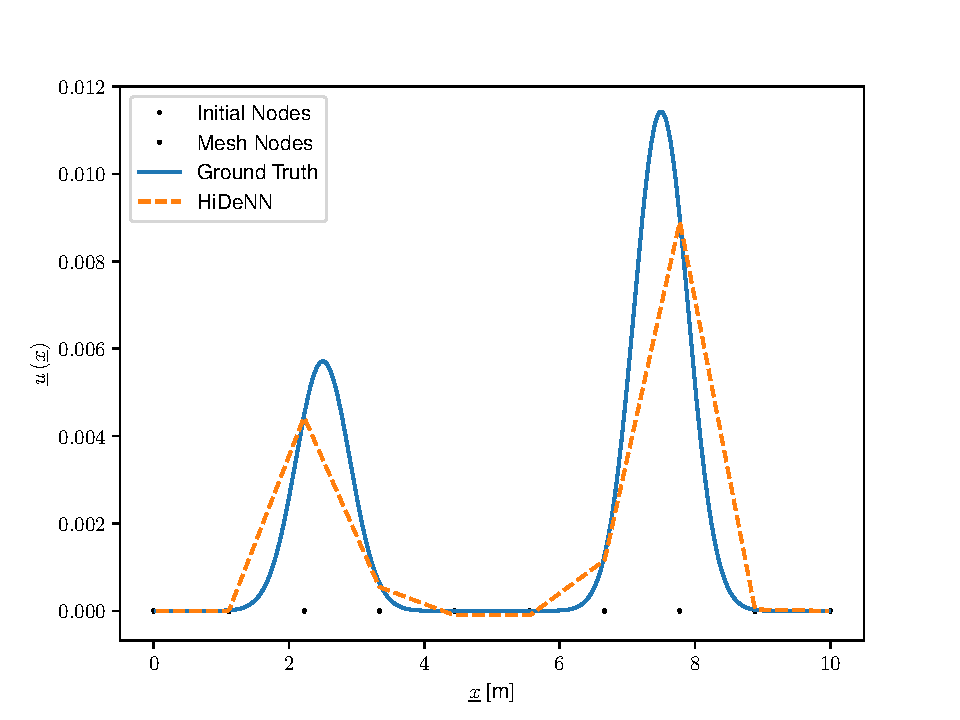
\includegraphics[width=\linewidth]{Figures/Solution_displacement_10_Frozen.pdf}
        \caption{Displacement}
    \end{subfigure}
    \begin{subfigure}{0.3\linewidth}
        \centering
        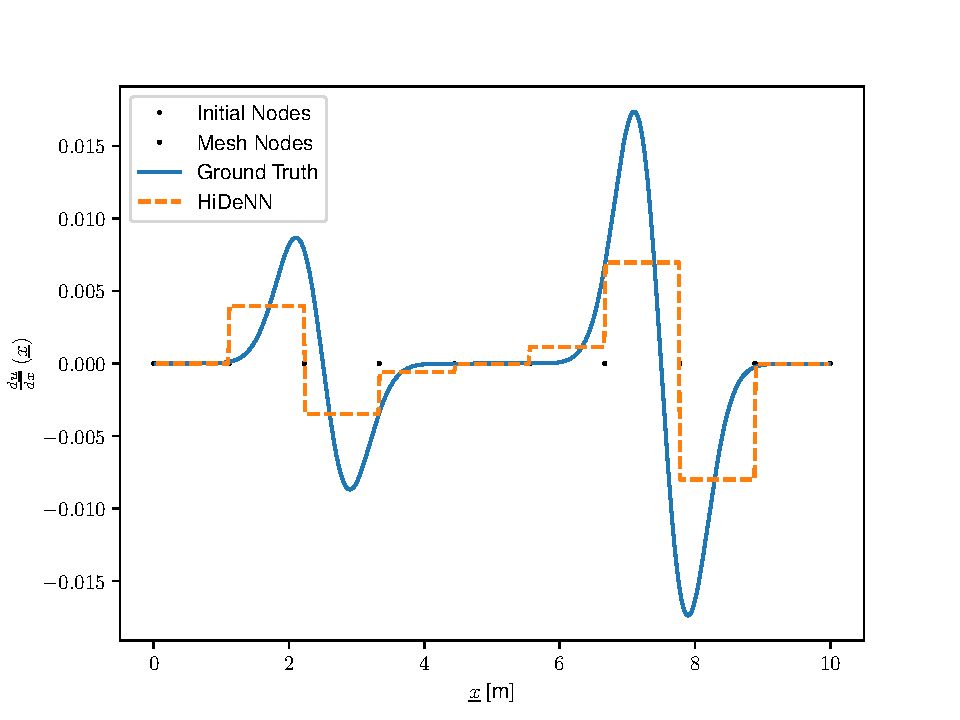
\includegraphics[width=\linewidth]{Figures/Solution_gradients_10_Frozen.pdf}
        \caption{Gradient}
    \end{subfigure}
    \caption{Frozen mesh - $n_p=10$}
    \label{fig:Fixed_Mesh10Float64}
\end{figure}

\begin{figure}
    \begin{subfigure}{0.3\linewidth}
        \centering
        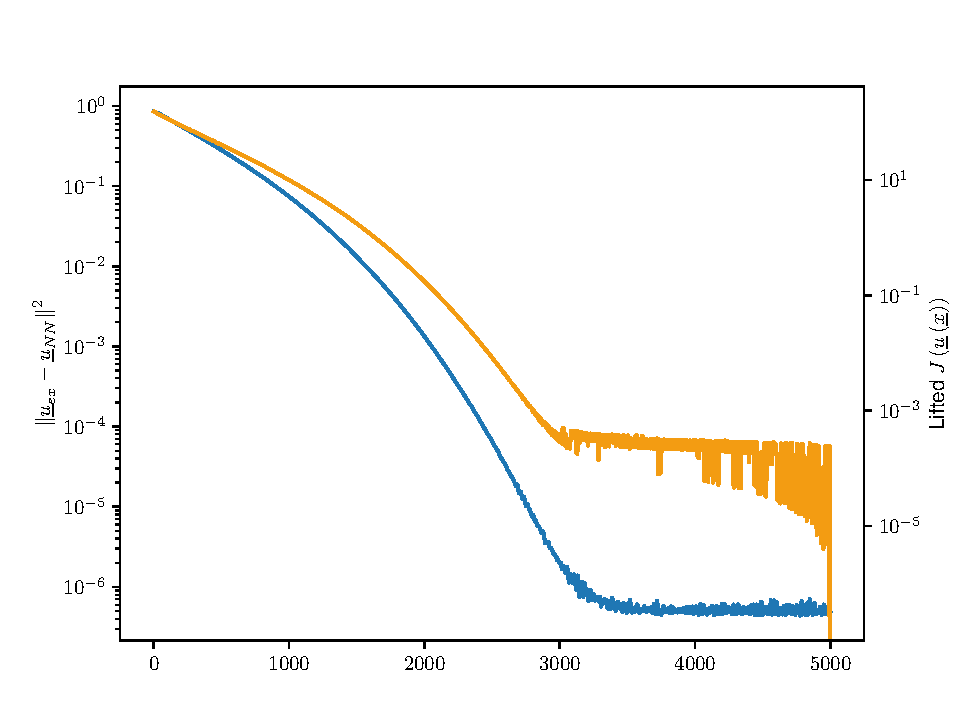
\includegraphics[width=\linewidth]{Figures/Loss_Comaprison_10_Regul.pdf}
        \caption{Evolution of the loss}
    \end{subfigure}
    \begin{subfigure}{0.3\linewidth}
        \centering
        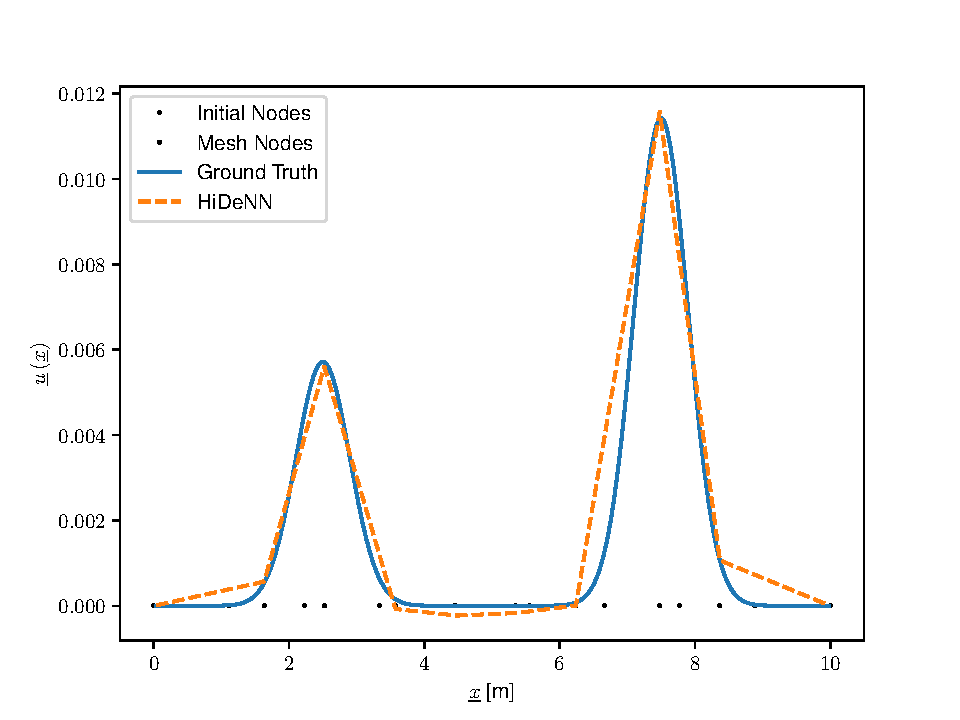
\includegraphics[width=\linewidth]{Figures/Solution_displacement_10_Regul.pdf}
        \caption{Displacement}
    \end{subfigure}
    \begin{subfigure}{0.3\linewidth}
        \centering
        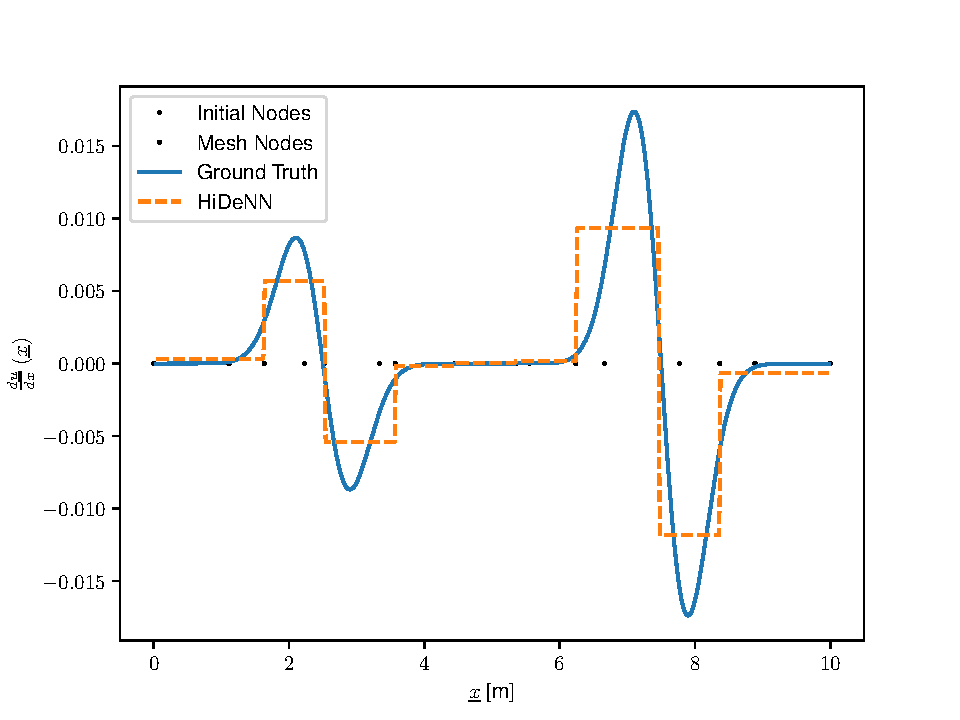
\includegraphics[width=\linewidth]{Figures/Solution_gradients_10_Regul.pdf}
        \caption{Gradient}
    \end{subfigure}
    \caption{Free mesh - $n_p=10$}
    \label{fig:Free_Mesh10Float64}
\end{figure}
% \chapter[The 1$^{\text{st}}$ of February 2024 - Architecture of the HiDeNN]{Architecture of the HiDeNN}

\begin{chapabstract}
    The question about a nodal-based or  an element-based architecture is discussed.
\end{chapabstract}

\minitoc

\section{Element-wise architecture}

When moving from linear 1D elements to higher order or dimensions, the use of an element-wise architecture \parencite{liu_hidenn-fem_2023} appears more versatile. The shape functions are therefore built on each element as opposed to globally on the mesh. 

One way of combining those approaches would be to add an \emph{Assembly layer} before the interpolation layer that rebuilds the global shape functions at the structure's (mesh) scale as illustrated in \cref{fig:assembly}.

For each element, a sub-neural network would be built so that the output consists of the local shape functions $\Tilde{N}_i$ defined on the element. 

% \paragraph{Warning} At this point, several versions of the same shape function (associated to the same node) can exist independently through different elements.
\Rq{At this point, several versions of the same shape function (associated to the same node) can exist independently through different elements.}

The \emph{Assembly layer} layer would then reconnect every local version $\Tilde{N}_i$ of a given global shape function $N_i$ associated to the $i-\text{th}$ node of the mesh. This layer would be a linear layer (\textbf{with bias of $-1$}) that inputs all the $\Tilde{N}_i$ and outputs a smaller layer of the $N_i$.
The weight matrix of such a layer would read
\begin{equation}
    w_{i,d\left(e-1\right)+k} = \begin{cases}
        1,\text{ if }k-\text{th node of element }e\text{ is node }i \\
        0,\text{ otherwise}
    \end{cases}
\end{equation}

\begin{figure}[bpt]
    \centering
    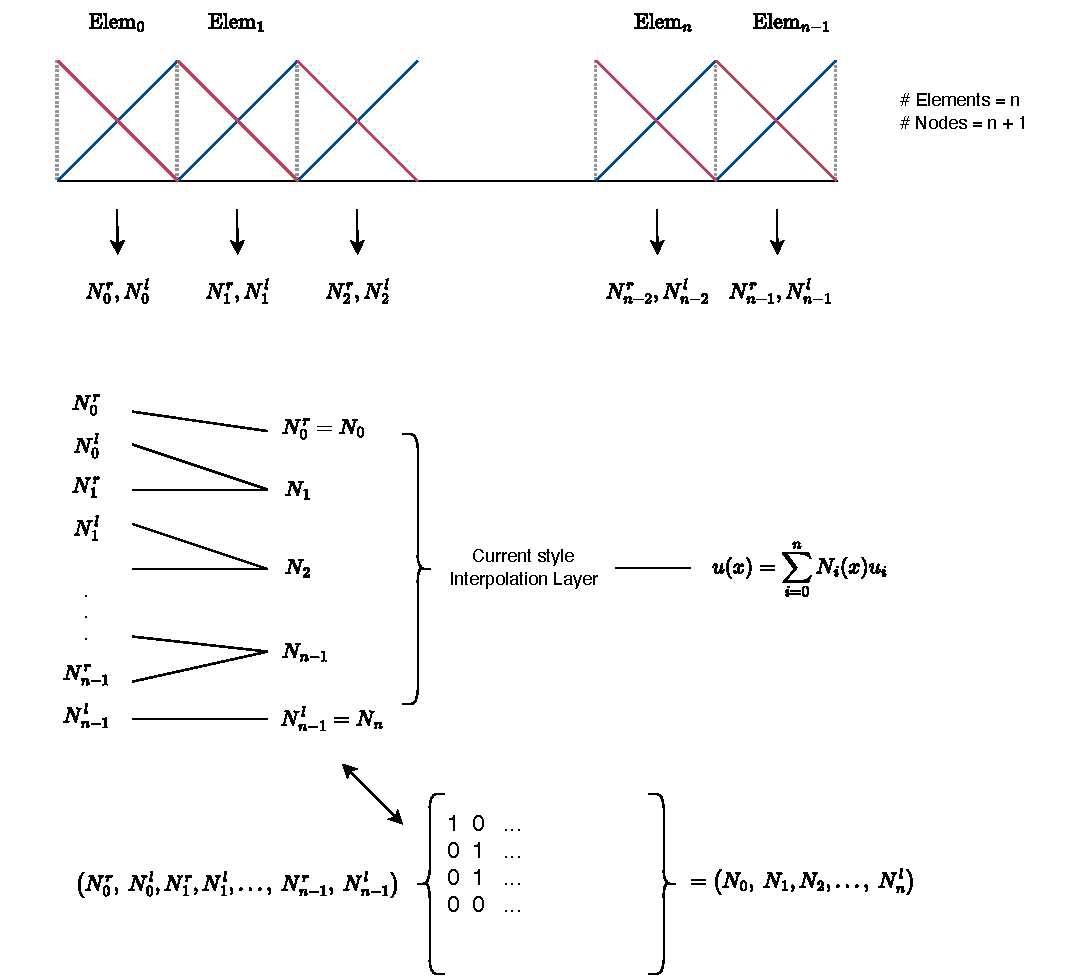
\includegraphics[width = 0.8\linewidth]{Schema/Diagram_NN_elementwise.drawio.pdf}
    \caption{Composition of shape functions.  The operation can be implemented using a linear layer with a weight matrix based on the connectivity table of given mesh and zero bias. This would allow using the existing interpolation layer consisting of nodal values.}
    \label{fig:assembly}
\end{figure}

% \paragraph{Warning}
% When decomposition the shape functions and then assembling them, using an element-wise support for the functions leads to issues on the exact nodal coordinates for the assembled global shape functions as illustrated in \cref{fig:Discontinuous}.


\begin{figure}[htbpt]
    \centering
    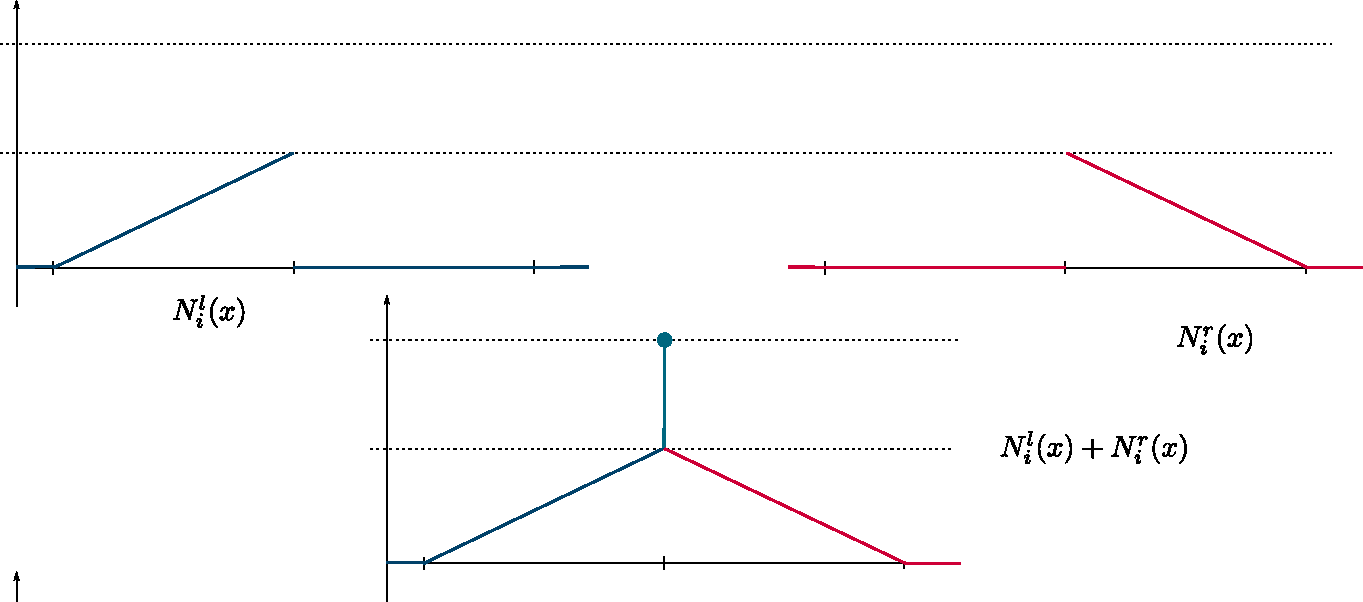
\includegraphics[width=\linewidth]{Schema/Discontinuous_sum.pdf}
    \caption{Element-wise support, discontinuous sum}
    \label{fig:Discontinuous}
\end{figure}
\Rq{When decomposition the shape functions and then assembling them, using an element-wise support for the functions leads to issues on the exact nodal coordinates for the assembled global shape functions as illustrated in \cref{fig:Discontinuous}.
}

Using ``leaking''shape functions that are defined outside of the element \parencite{zhang_hierarchical_2021} allow to bypass this issue as shown in \cref{fig:Continuous}. In that case the assembly layer will need to have the $-1$ biais shown in the last layer of the shape functions detailed by \cite{zhang_hierarchical_2021}.
\begin{itemize}
    \item[\faLightbulb] Check how to apply that idea in higher dimensions
\end{itemize}
\begin{figure}[hbpt]
    \centering
    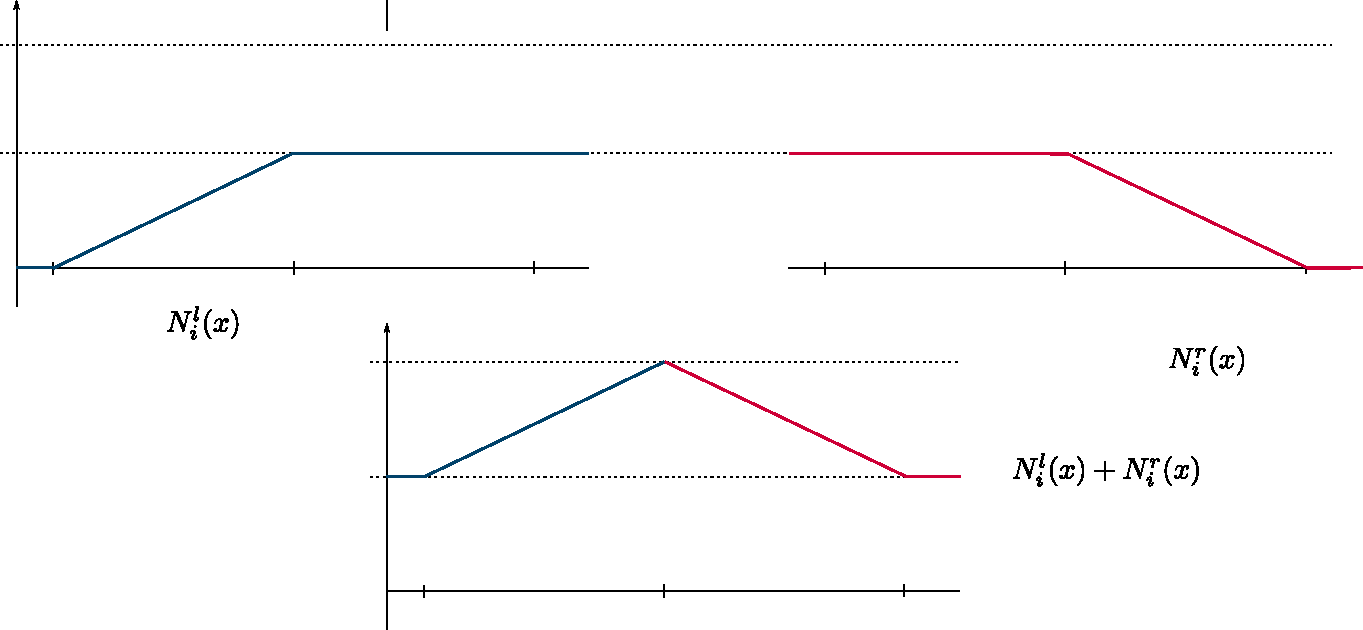
\includegraphics[width=\linewidth]{Schema/Continuous_sum.pdf}
    \caption{Leaking shape functions, continuous sum}
    \label{fig:Continuous}
\end{figure}

\section{Parametric implementation}
The benefits of HiDeNN seem to lie in the parametric capability of such architectures. See \cref{chap:TD}.
\Rq{\begin{itemize}
    \item Feels like without parameters there are no real advantages of HiDeNN over solving the finite element problem
    \begin{itemize}
        \item Maybe in cases where extreme re-meshing is required
    \end{itemize}
    \item With parameters and Tensor Decomposition, the decomposition could be easily automated (might be better than fixed point)
    \begin{itemize}
        \item They sell a parametric version of HiDeNN but so far the only parameters are the 3 spatial parameters (even for HiDeNN-TD) \faChevronRight ~no real ROM yet
    \end{itemize}
    \item Achieve new kind of \emph{a priori} ROM (no snapshots required)
    \item Could get non-linear interpolation relatively "easily"
\end{itemize}}
%\chapter[The 6$^{\text{th}}$ of February 2024 - Method papers - Goals \& quick description]{Method papers - Goals \& quick description}
\label{chap:MethodPapers}
\begin{chapabstract}
    The chapter recaps the meeting where we outline the objectives of the two method papers we aim to submit before summer.
\end{chapabstract}

\minitoc

\section{Method papers}

The first objective of 2024 is to set up the required tools to speed up both the micro and macro problems. The HiDeNN framework \parencite{zhang_hierarchical_2021} is a suitable candidate to give reduced models at both scales.

Some developments are still required to have a suitable framework for our needs. These developments are expected to be promoted through two \emph{method papers} described in the following sections.

\section{PDE solving - Mixed formulation}
The objective of that first paper would be to present
\begin{itemize}
    \item Optimised training strategy 
    \item Use a Mixed-formulation (PINN form of loss function)
    \item ``Element-wise'' implementation
\end{itemize}

Some open questions / possible work could include working on 
\begin{itemize}
    \item Regularisation of the Loss / Preventing collision of the nodes (negative Jacobian) to occur
\end{itemize}

The closest milestones are
\begin{itemize}
    \item Quadratics shape functions in 1D
    \item Definitions of shape functions suitable for 2D (see \cref{chap:TD})
\end{itemize}

\section{Parametric PDE}

An essential aspect of the required tool is providing a reduced-order parametric field model. 
\subsection{Short term}
This paper will rely on the tensor decomposition (TD) presented by \cite{zhang_hidenn-td_2022} and described in \cref{chap:TD}. It will focus on 
\begin{itemize}
    \item Implementing different parameters in the TD (as opposed to only spatial parameters as in \parencite{zhang_hidenn-td_2022}).
    \item Adapt the number of modes of the tensor decomposition of the fly (\emph{a priori ROM})
    \item Automate the non-linear interpolation using non-linear combinations of the modes (as opposed to solely using linear combinations of the modes as done in PGD, for instance)
    \begin{itemize}
        \item Such an optimisation could be based on a fully connected small NN in between the modes and the solution layer.
        \item $\vect{u}\left(\textcolor{BleuLMS!70}{\vect{x}}, \textcolor{LGreenLMS}{\left\{\mu_i\right\}_{i \ in \llbracket 1, \beta \rrbracket}}\right) = \sum\limits_{i=1}^m \textcolor{BleuLMS!70}{f\left(\overline{\vect{u}}_i(\vect{x})\right)} ~\textcolor{LGreenLMS}{\prod_{j=1}^{\beta}g\left(\lambda_i^j(\mu^j)\right)}$ 
        With $f$ and $g$ arbitrary functions of the modes, learned by the neural network in the reduced-order space so that the learning cost is lower but we achieve better reductibility by using non-linear combinations of the modes instead of increasing drastically the number of modes required.
        \item Take up the general idea put forward by \cite{kramer_learning_2024,geelen_learning_2023} but extend it to automate the non-linear combination  without prior knowledge of the required interpolation as opposed to guessing polynomial combinations
    \end{itemize}
\end{itemize}

A nice bonus would include the aspects of parametric spatial dependency described in \cref{chap:TD} in \cref{sec:SpatialParameters}.

\subsection{Mid term}
\label{ParaRefinement}
If the parameters' space is a tensor product of 1D spaces, then a localised refinement (as illustrated in \cref{fig:LocalRefinement}) of the parametric space is impossible, which would render the parametric description too heavy (as illustrated in \cref{fig:TDRefinement}). A specific strategy to describe the parameter space is required for localised refinement. 
\begin{itemize}
    \item High dimension shape functions for the hypercube parameters for instance
    \item What would be the impact of a pre-processing fully connected layer in between the input of the parameters and the 1D shape functions of the parameters?
    \begin{itemize}
        \item The parameters would not be treated independently from one another anymore as the pre-processing layer would connect them. What impact would that have on the Tensor Decomposition?
    \end{itemize}
\end{itemize}

\begin{figure}
\begin{subfigure}[t]{0.5\linewidth}
    \centering
    	\begin{tikzpicture}[scale=1.5]
		
		 % Orthonormal frame of reference
		\draw[->] (0,0) -- (4.5,0) node[below right] {$\mu_1$};
		\draw[->] (0,0) -- (0,3.5) node[above left] {$\mu_2$};
		
		% Draw coarse mesh
		\foreach \x in {0,1,2,3}{
			\foreach \y in {0,1,2}{
				\draw[BleuLMS] (\x,\y) rectangle (\x+1,\y+1);
			}
		}
		
		% Refinement region
		\draw[GreenLMS, very thick] (1,1) rectangle (2,2);
		
		% Draw refined mesh
		\foreach \x in {1}{
			\foreach \y in {1}{
				\draw[GreenLMS, thick] (\x,\y) rectangle (\x+0.5,\y+0.5);
			}
		}
				\foreach \x in {1.5}{
			\foreach \y in {1.5}{
				\draw[GreenLMS, thick] (\x,\y) rectangle (\x+0.5,\y+0.5);
			}
		}
		
		% Draw rerefined mesh
		\foreach \x in {1}{
			\foreach \y in {1}{
				\draw[GreenLMS, thick] (\x,\y) rectangle (\x+0.25,\y+0.25);
			}
		}
		\foreach \x in {1.25}{
	\foreach \y in {1.25}{
		\draw[GreenLMS, thick] (\x,\y) rectangle (\x+0.25,\y+0.25);
	}
}

	\end{tikzpicture}
    \caption{Local refinement in a 2D parametric space}
    \label{fig:LocalRefinement}
\end{subfigure}
  \begin{subfigure}[t]{0.5\linewidth}
    \centering
    	\begin{tikzpicture}[scale=1.5]
		
		% Orthonormal frame of reference
		\draw[->] (0,0) -- (4.5,0) node[below right] {$\mu_1$};
		\draw[->] (0,0) -- (0,3.5) node[above left] {$\mu_2$};
		
		% Draw coarse mesh
		\foreach \x in {0,1,2,3}{
			\foreach \y in {0,1,2}{
				\draw[BleuLMS] (\x,\y) rectangle (\x+1,\y+1);
			}
		}
		% Refinement region
		\draw[GreenLMS, very thick] (1,1) rectangle (2,2);
		\foreach \y in {0,1,2}{
		\draw[BleuLMS] (1,\y) rectangle (1.25,\y+1);
		}
		\foreach \y in {0,1,2}{
			\draw[BleuLMS] (1.5,\y) rectangle (2,\y+1);
		}
		
		\foreach \x in {0,1,2,3}{
			\draw[BleuLMS] (\x,1) rectangle (\x+1,1.25);
		}
		\foreach \x in {0,1,2,3}{
			\draw[BleuLMS] (\x,1.5) rectangle (\x+1,2);
		}
	

	\end{tikzpicture}
    \caption{Constrained refinement in two 1D-spaces tensor product}
    \label{fig:TDRefinement}
\end{subfigure}  
\caption{Refinement possibility of a 2D parametric space compared to its counterpart decomposed as a tensor product of two 1D spaces}
\end{figure}

\Rq{Each PGD modes are computed on an independent mesh, hence the localised correction of latter modes can lead to specific mesh refinement. \newline \noindent \textcolor{LGreenLMS}{\faLightbulb} This could solve the issue mentioned above.}
% \chapter[The 29$^{\text{th}}$ of February 2024 - Parametric investigation]{Parametric investigation}
\begin{chapabstract}
    Recaps of the novelty and investigations: 2- and 3-parameter NN-PGD
\end{chapabstract}

\minitoc

\section{NeuROM - Parametric reduced-order model}
\subsection{1 extra parameter}
Varying the overall stiffness on the hole structure.
\begin{itemize}
    \item First implementation of a NN-PGD (not automatically Greedy yet) \cref{chap:TD} in \cref{1D_NeuROM}
    \begin{itemize}
        \item The error indicator provided by the mixed formulation might be useful for on the fly decision of addition of new modes or not
    \end{itemize}
    \item Might need to rethink the Module architecture if no way to parallelise using \code{vmap} (Vectorisation of Modules).
    \item Advantage of classical PGD, only the loss has to be re-written for a new problem
    \item Initialisation from coarser ROM (coarser mesh and/or fewer modes) in \cref{chap:Transfer_learning}.
    \begin{itemize}
        \item In the same spirit as \cite{giacoma_toward_2015}
        \item Leverage higher transfer learning capabilities of HiDeNN
    \end{itemize}
    \item Discussion on the orthogonality constraint 
    \item Non zero BCs implementation in NeuROM in \cref{chap:TD} in \cref{BCs_TD}
    \item Different behaviour with non zero BCs
\end{itemize}

\subsection{2 extra parametera}

Works very well (3 modes) for a 2 stiffness structure (left half and right half having different young moduli that can each take any given value in a given parametric range. (how to represent without GiF ?) \cref{chap:TD} in \cref{1D_NeuROM_Bi}
\section{Technical}

\subsection{Code efficiency}

\begin{itemize}
    \item Re-think architecture to vectorise as many functions as possible
    \item Need to use GPUs to get same performaces as FEM solvers \parencite{park_convolution_2023}
\end{itemize}

\subsection{Jean-Zay cluster}

See \cref{chap:Note} in \cref{sec:JZ}.


% \chapter[The 8$^{\text{th}}$ of March 2024]{}
\minitoc
\section{Mixed formulation}
\subsection{To do}
\begin{itemize}
    \item Recompute the experiments with $\alpha=0.0$. We don't need to Jacobian-based regularisation at the moment and since everything is super sensitive, it might make a difference in the results.
    \item Use normalised version of the $l_2$ error.
    \begin{itemize}
        \item In the parametric version, the computation of the normalised $\mathcal{L}_2$ error is already implemented
    \end{itemize}
\end{itemize}

\subsection{To think about}
\begin{itemize}
    \item How could we share the mesh for $u$ and $du$? We want the mesh coordinates to be effected by both loss terms. Also, some of the nodes are not shared by both variables. How to deal with this in our code?
    \item Is mixed-formulation solution equal to exact solution at the mesh nodes?
\end{itemize}

\section{2D domain }
\subsection{To do}
\begin{itemize}
    \item Triangular mesh. 
    \item Implement the reference element. For each training point $x$, find cell ID $i$. For cell $i$, get the coordinates of nodes and compute $L_i$ coordinates. Based on them, get the position of $x$ in reference element - $\xi$. Evaluate the shape functions, defined on the reference element, for $\xi$. Do the interpolation. \emph{I need to study the details. }
    
\end{itemize}

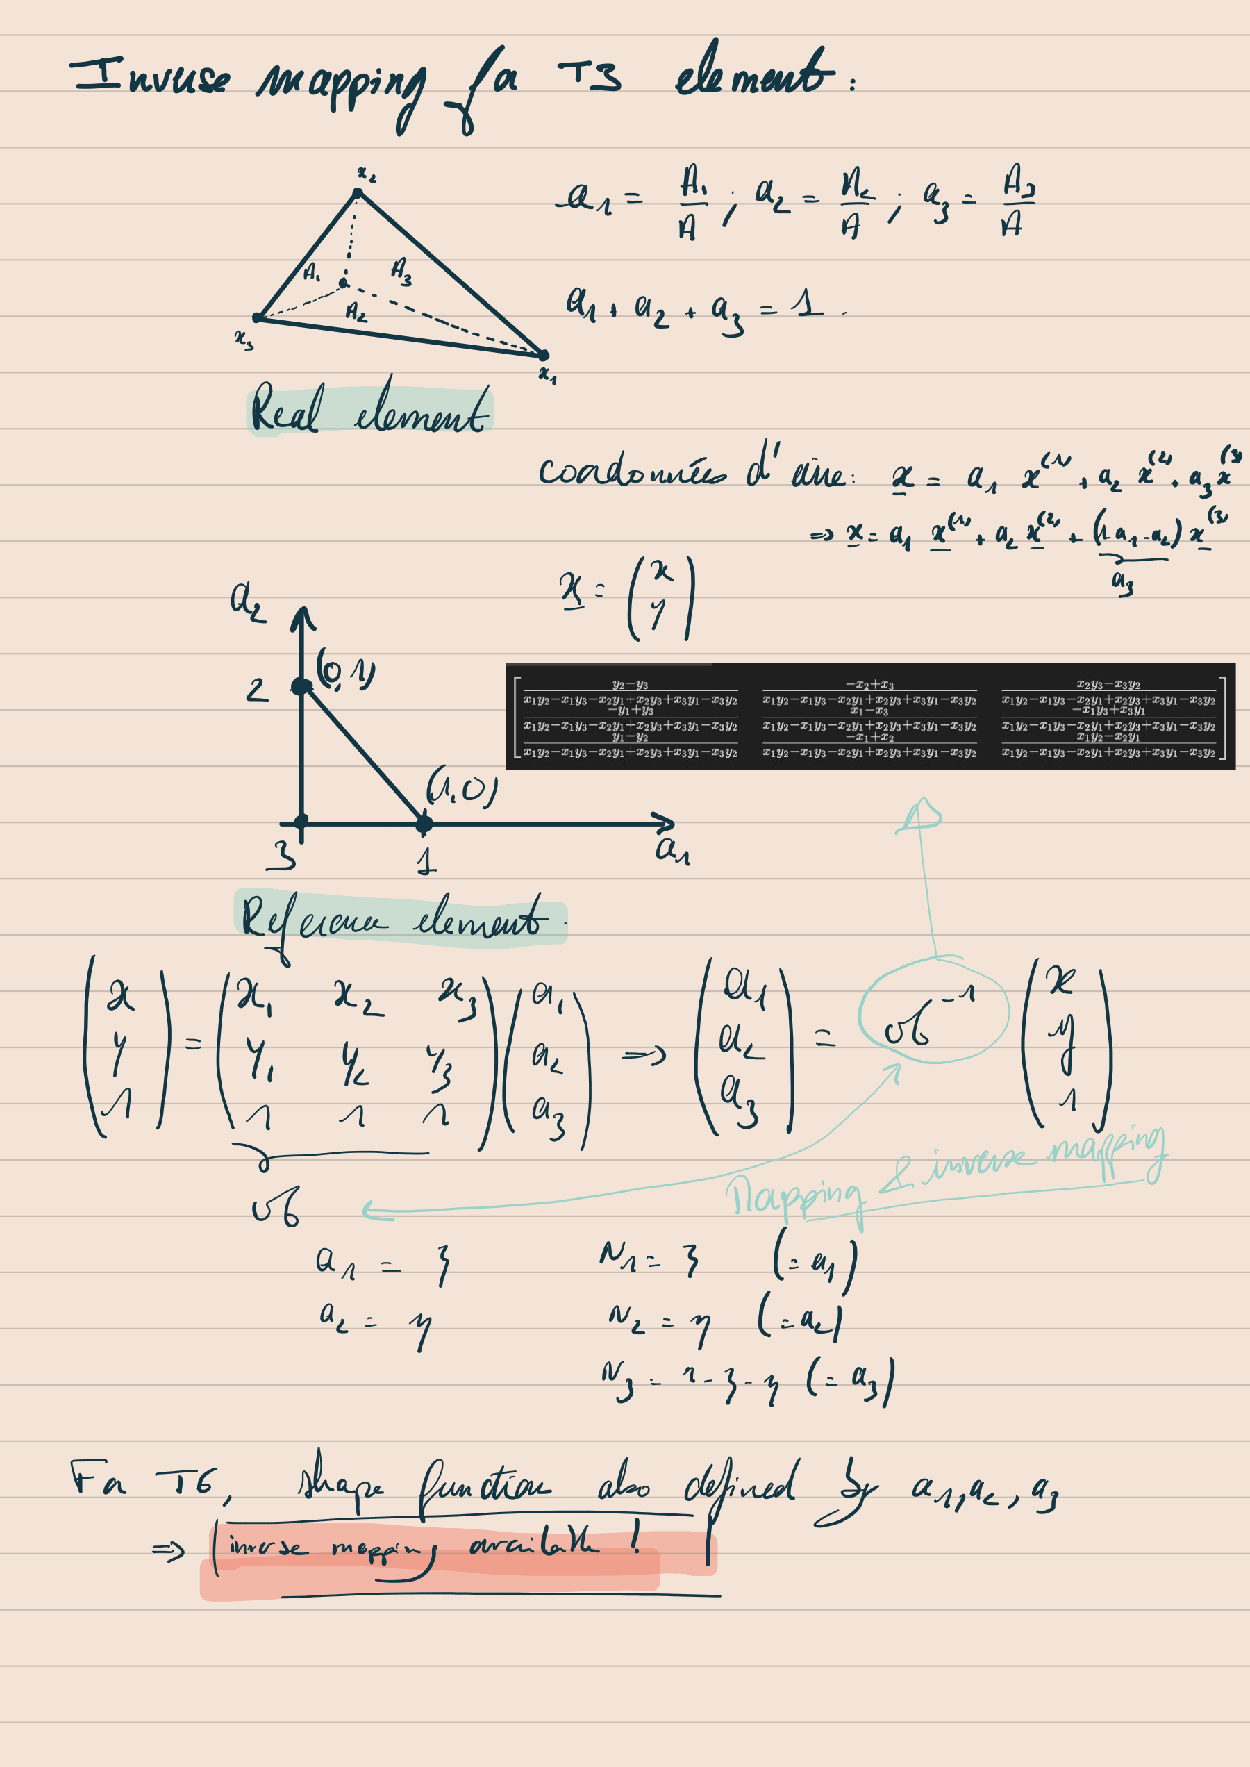
\includepdf[pages={1}]{Figures/InverseMappingT3.pdf}

\section{TODO Parametric}

\begin{itemize}
    \item Multi scale Tensor decomposition (Since modes can live on different meshes)
    \item Non-linear interpolation
    \item Non-linear potential to minimise
    \item Using mixed formulation
\end{itemize}
\section{``Big picture''}

If we can make this tool robust, it can dissociate the interpolation aspect from the solving of the PDE and give access to a high level tool in the sens that coding a solver would not be required but only writing the expression of the loss would be needed.

\begin{itemize}
    \item In the same sens that no one codes a linear solver but uses linear algebra libraries this be used as a replacement for non linear solvers with mesh adaptivity and parametric representation built into it
    \item Allow to use tensor decomposition and other technique without having to explicitly write the linearised problem and the iterative non-linear solver
    \item TODO: investigates its behaviour regarding snap-back and snap-through problems
\end{itemize}

\chapter[The 22$^{\text{nd}}$ of March 2024 - 2D and Orthogonality discussion]{2D and Orthogonality discussion}
\label{Chap_22_03_24}
\begin{chapabstract}
    This week the 2D has drastically moved forward and some investigations on the orthogonality were made. 
\end{chapabstract}

\minitoc

\section{2D}

The mixed formulation with T3 elements works. Quadratic elements are on the way

\section{Orthogonality}
\label{sec:orthogonality}
 In order for the loss implementation not to somehow bring back the curse of dimensionality it is important to rely on the tensor decomposition and not compute the full order tensors. However, it does not seem easy to remove the full tensors field evaluation to compute the integral due to the square of the gradient 
 \begin{equation}
     \left( \frac{\partial u}{\partial x} \right)^2 = \left( \sum\limits_{i=1}^m \textcolor{BleuLMS!70}{\frac{\mathrm{d}\overline{\vect{u}}_i(\vect{x}) }{\mathrm{d}x}} ~\textcolor{LGreenLMS}{\prod_{j=1}^{\beta}\lambda_i^j(\mu^j)} \right)^2.
 \end{equation}
 To do so an idea could be to try to rely on  the orthogonality of the space modes.
 
\subsection{Post processing Gram-Schmidt}
So as not to modify the interpolation given by the NN, it appears less intrusive to solely modify the post-processing of the interpolated field before computing the loss.

\subsubsection{One extra parameter}
An orthogonalisation step can be carried out in the case of a single extra-coordinate. This step allows the previously computed modes to form a basis without losing the newly computed information. Moreover, projecting a new mode onto the basis provides additional insights: the extent to which it adds new information. For instance, if its projection is zero, it indicates that the previous modes already represent this mode, rendering it irrelevant. In practical terms, for each pair of modes $\left(\overline{\vect{u}}_{m+1},\lambda_{m+1}\right)$, we ``eliminate" from $\overline{\vect{u}}_{m+1}$ the projection of the new mode onto the preceding modes, yielding $\mathring{\overline{\vect{u}}}_{m+1}$. Consequently, we adjust the $\lambda_{i}$ values accordingly to avoid information loss, resulting in $\mathring{\lambda}_i$. Subsequently, we normalise this new mode $\mathring{\overline{\vect{u}}}_{m+1}$ using equations (\ref{ortho}), (\ref{normaliz1}), (\ref{normaliz2}), and (\ref{normaliz3}).
	
	\begin{equation}\label{ortho}
		\vect{u}_{m+1} = \sum_{i=1}^{m} \underbrace{(\lambda_i + \lambda_{m+1} ~ \overline{\vect{u}}_i^T  \overline{\vect{u}})}_{\mathring{\lambda}_i} \overline{\vect{u}}_i + \lambda_{m+1} \underbrace{\left(\overline{\vect{u}}_{m+1} - \sum_{i=1}^{m} ( \overline{\vect{u}}_i^T  \overline{\vect{u}}) \overline{\vect{u}}_i\right)}_{\mathring{\overline{\vect{u}}}_{m+1}}
	\end{equation}
	
	\begin{equation}\label{normaliz1}
		\overline{\vect{u}}_{m+1} \longleftarrow \frac{\mathring{\overline{\vect{u}}}_{m+1}}{\Vert\mathring{\overline{\vect{u}}}_{m+1} \Vert_{\ftensor{K}}}
	\end{equation}
	
	\begin{equation}\label{normaliz2}
		\lambda_{m+1} \longleftarrow \lambda_{m+1} \Vert\mathring{\overline{\vect{u}}}_{m+1} \Vert_{\ftensor{K}}
\end{equation}
\begin{equation}\label{normaliz3}
	\{\lambda_i\}_{i\in\llbracket1,m\rrbracket} \gets \{\mathring{\lambda}_i\}_{i\in\llbracket1,m\rrbracket}
\end{equation}
\Rq{Alternatively, time vectors can also be compressed as proposed in \parencite{giacoma_toward_2015}, converging towards the SVD decomposition of the displacement field, thus avoiding redundancy in temporal vectors.}


\subsubsection{Multiple extra parameters}

The modified Gram-Schmidt algorithm that allows keeping the same solution field after and before the orthonormalisation process is not applicable in case of more than 1 extra parameter. Indeed, orthogonalising the mode $m+1$ with the previous basis without loosing information amounts to writing 
	\begin{equation}\label{ortho}
		\vect{u}_{m+1} = \sum_{i=1}^{m} \underbrace{(\lambda_i^{(1)}\lambda_i^{(2)} + \lambda_{m+1}^{(1)}\lambda_{m+1}^{(2)} ~ \overline{\vect{u}}_i^T  \overline{\vect{u}})}_{\neq \mathring{\lambda}_i^{(1)}\mathring{\lambda}_i^{(2)}} \overline{\vect{u}}_i + \lambda_{m+1}^{(1)}\lambda_{m+1}^{(2)} \underbrace{\left(\overline{\vect{u}}_{m+1} - \sum_{i=1}^{m} ( \overline{\vect{u}}_i^T  \overline{\vect{u}}) \overline{\vect{u}}_i\right)}_{\mathring{\overline{\vect{u}}}_{m+1}}.
	\end{equation}
In the general case, 
\begin{equation}
    (\lambda_i^{(1)}\lambda_i^{(2)} + \lambda_{m+1}^{(1)}\lambda_{m+1}^{(2)} ~ \overline{\vect{u}}_i^T  \overline{\vect{u}}) \neq \mathring{\lambda}_i^{(1)}\mathring{\lambda}_i^{(2)}.
\end{equation}

The corrected previous modes cannot be written as a single modifed mode but must stay a tensor decomposition of dimension $\beta$ ($\beta$ being the number of extracoordinates),rendering the tensor decomposition moot after the orthogonalisation process since it preserves the curse of dimensionality removing only the space dimension.

\subsection{Orthogonalisation process within the interpolation NN}

In order to get passed the previously seen limitation, an idea could be to pass the ram-Schmidt (GS) algorithm earlier in the NN before the combination of the space modes and parameter modes as illustrated in \cref{fig:GS_NN}. Doing so means that the parameter modes are directly computed on the orthonormal basis therefore there is no need to modify them afterwards to match the new orthonormal basis.

\begin{figure}
    \centering
    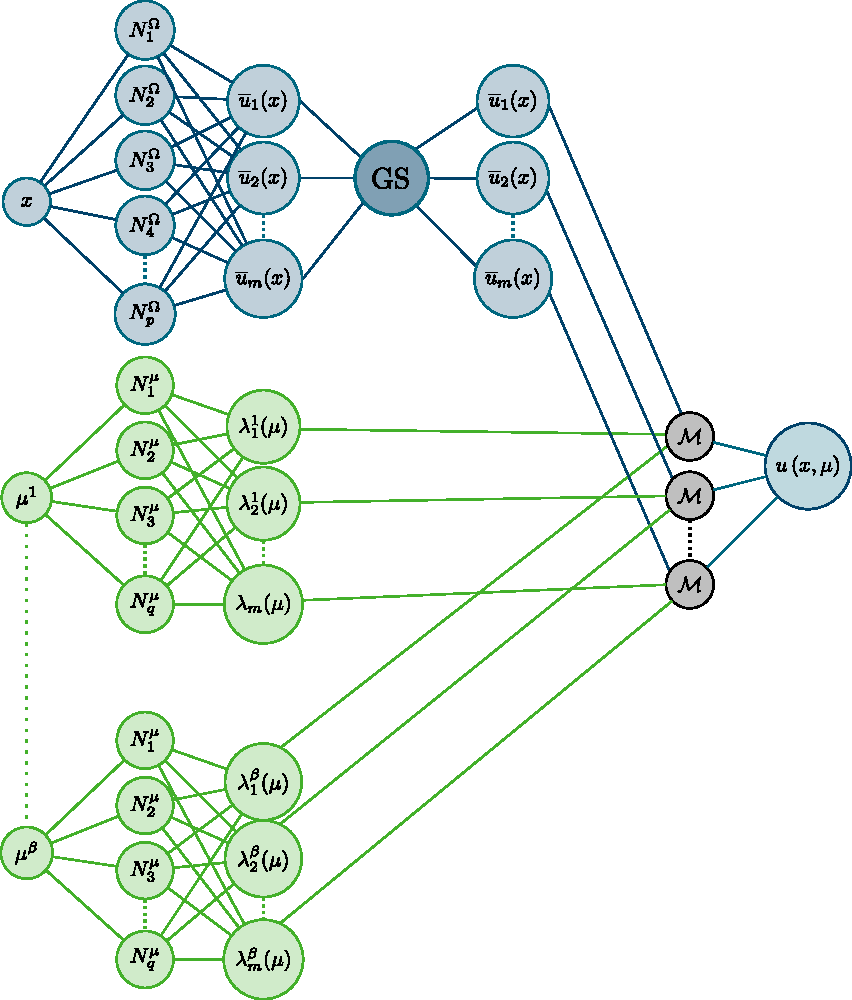
\includegraphics[width = 0.8\textwidth]{Schema/GramSchmidt_NN.pdf}
    \caption{Gram-Schmidt within the HiDeNN-PGD}
    \label{fig:GS_NN}
\end{figure}

\paragraph{This was a bad idea}
It does make sens to orthonomalise the $\left\{ \vect{u}\left( x_i \right) \right\}_{ i \in \llbracket 1, s \rrbracket}$ (with $s$ the number of sampling points) within the NN because it will then depend on the size of the input batches.
Adding a GS algorithm on the \emph{interpolated} space modes (whose size depends on the number of sampling point) only makes sens as a post-process when computing the loss if the training sample is always the same. But this does not seem feasible with more than 1 extra coordinate.

\Rq{The key difference with classical ROM is that not only there are ``Nodally defined'' space modes that lives on the mesh as classically encountered in ROM but there are also the interpolated continuous space modes that are evaluated at the sampling points when evaluating the NN. The latter are the one we play with the most and there interpretation and the operation that can be done on those differ from what is standard on the ``nodal modes'' }

% \chapter[The 15$^{\text{th}}$ of March 2024]{2D and efficiency investigations}
\begin{chapabstract}
    This week the 2D has drastically moved forward and some investigations on the efficiency of the parametric investigation were made.
\end{chapabstract}

\minitoc

\section{2D}

\begin{itemize}
    \item Reference elements are implemented for T3 element
    \item Boundary conditions are implemented and automated
    \begin{itemize}
        \item Small strain only, no normal vector computation yet
    \end{itemize}
\end{itemize}



\section{Parametric efficiency}

\subsection{Efficiency findings}
When the number of parameters increases the cost drastically increases and I do not know why. 


\subsection{Different implementation strategies}
Basically the parameters and the modes are handled as a list of Modules (functions) that are indexed by the mode number and the parameter number. Each function within the list is well vectorised.


\paragraph{The first non optimal idea is to use for loops}

Two nested loops to iterate through the functions stored in \code{self.Para\_modes}.
\RestyleAlgo{ruled}

%% This is needed if you want to add comments in
%% your algorithm with \Comment
\SetKwComment{Comment}{/* }{ */}
\SetEndCharOfAlgoLine{}
\begin{algorithm}[hbtp!]
	\caption{Parameter modes evaluation}\label{alg:two}
	\textbf{Inputs: } \code{Para\_mode\_Lists}, \code{mu} \textcolor{GreenLMS}{\Comment*[r]{List of Modules and parameters samples mu}}
	
	\For(\textcolor{GreenLMS}{\Comment*[r]{\hspace{-5pt}Loop over the modes\hspace{-6pt}}}){$k \in \llbracket 1,m \rrbracket$}{

	\For(\textcolor{GreenLMS}{\Comment*[r]{\hspace{-5pt}Loop over the parameters\hspace{-6pt}}}){$k \in \llbracket 1,\beta \rrbracket$}{
            \code{Para\_mode\_Lists[mode][l] = self.Para\_modes[mode][l](mu[l]) 
            }
    }
    }
\end{algorithm}

\paragraph{List comprehension}

The for loops can easily be converted to list comprehension.

\begin{algorithm}[hbtp!]
	\caption{Parameter modes evaluation}\label{alg:two}
	\textbf{Inputs: } \code{Para\_mode\_Lists}, \code{mu} \textcolor{GreenLMS}{\Comment*[r]{List of Modules and parameters samples mu}}
	
\code{Para\_mode\_Lists = [[self.Para\_modes[mode][p](mu[p])} 
\code{for p in range(self.n\_para)]for mode in range(self.n\_modes)]}
\end{algorithm}

No speed-up is observed. The \code{ModuleList} offers the same syntax as python lists but the implementation might differ.

\paragraph{Vectorisation over the indexes} Because the output of each functions in \code{ModuleList} are independent from one-another it would be perfectly possible to run their evaluation in parallel. To that aim several vectorisation implementation where tried with little to no success.

\begin{itemize}
    \item Slicing does not work on Module or function lists
    \item There's no way to vmap directly over an array of functions \href{https://github.com/google/jax/issues/673}{see this topic}
    \item There is a workaround using switch (not implemented in \textsc{pytorch} yet but works with jax)
\end{itemize}

I tried the workaround proposed \href{https://github.com/google/jax/issues/673}{here} using jax to compare the speed up results and.... it was way worse (10x slower than using for loops).

I tried \code{jax.jit} over the vmaped function and it was even worse (100x slower than using for loops)

\Rq{Those findings might be linked to early versions of jax not being well optimised for M2 chips yet}


\paragraph{Results:}
On a simpler example the evaluation of the above mentioned methods was tried and yield the conclusion that on our hardware the list comprehension might be the best way to go.
\begin{verbatim}
**** Example 1 ****
For loop:               t = 1.180887222290039ms
List comprehension:     t = 1.0099411010742188ms
vmap:                   t = 100.78692436218262ms
\end{verbatim}


\paragraph{Investigation on why it is so slow}

with one parameter the complexity seems to be O(m) which sounds reasonable.

If I fix $m=1$ and go from $1$ parameter to $2$, the running time per epoch increases by a factor $5$.

\Rqs{It might be due to the loss implementation that somehow brings back the curse of dimensionality. It does not seem easy to remove the full tensors field evaluation to compute the integral due to the square of the gradient $$\left( \frac{\partial u}{\partial x} \right)^2 = \left( \sum\limits_{i=1}^m \textcolor{BleuLMS!70}{\frac{\mathrm{d}\overline{\vect{u}}_i(\vect{x}) }{\mathrm{d}x}} ~\textcolor{LGreenLMS}{\prod_{j=1}^{\beta}\lambda_i^j(\mu^j)} \right)^2$$}{Try to rely on  the orthogonality of the space modes (which we do not have currently but could be post-processed with GS or constrained )}

\subsection{TODO}
\begin{itemize}
    \item Greedy algorithm (based on mixed formulation error indicator)
    \item \textbf{Learn the number of modes with a sparsity constraint}
    \begin{itemize}
        \item Start with a fixed weight on the sparisity constraint 
        \item decrease the weight imposing sparsity if convergence is too slow
        \item Similar to update/adding modes criterion in PGD
    \end{itemize}
    \item Study on imposing or not orthogonality
    \item Gram Schimdt
    \item Non-linear interpolation using a deeper NN
\end{itemize}



\clearpage{\thispagestyle{empty}\cleardoublepage}
% % Part II
\part{Drafts - Notepad}
\input{chapters/Tensordecomposition.tex}
\chapter[Mixed Formulation]{Mixed formulation}
\label{chap:MixedFormulation}
\begin{chapabstract}
    This chapter investigates the implementation of a mixed formulation in the HiDeNN framework.
\end{chapabstract}

\minitoc

\section{Element wise architecture}

When moving from linear 1D elements to higher order or dimensions, the use of an element wise architecture appears more versatile. The shape functions are therefore built on each element as opposed to globally on the mesh. 

One way of combining those approaches would be to add an \emph{Assembly layer} layer before the interpolation layer that rebuilds the global shape functions at the structure's (mesh) scale.

For each element, a sub-neural network would be built so that the output consists on the local shape functions $\Tilde{N}_i$ defined on the element. 

\Rq{At this point, several versions of the same shape function (associated to the same node) can exist independently through different elements.}

The \emph{Assembly layer} layer would then reconnect every local version $\Tilde{N}_i$ of a given global shape function $N_i$ associated to the $i-\text{th}$ node of the mesh. This layer would be a linear layer (without bias) that inputs all the $\Tilde{N}_i$ and outputs a smaller layer of the $N_i$.
The weight matrix of such a layer would read
\begin{equation}
    w_{i,d\left(e-1\right)+k} = \begin{cases}
        1,\text{ if }k-\text{th node of element }e\text{ is node }i \\
        0,\text{ otherwise}
    \end{cases}
\end{equation}

\section{Continuous vs. Discontinuous global shape functions}

Contrary to what we though, we in fact need to use the "leaking" version of shape functions (see \cref{fig:Continuous}). This might complicate the composition of global shape functions in higher dimensions, as the problem of non-zero values outside given element can not be simply solved by subtracting a constant value. However, creating the discontinuous global shape functions (see \cref{fig:Discontinuous}) is not possible using differentiable functions.

 We might still consider using the filter in front of the neural network: for $x \neq x_i$, $u(x)$ is obtained by interpolation provided by the neural network; for $x \neq x_i$, $u(x)$ is obtained directly as $u_i$. This is not necessary to deal with the incorrect value of shape functions, but it wold help us avoid the problem with zero derivatives.

 
\begin{figure}
    \centering
    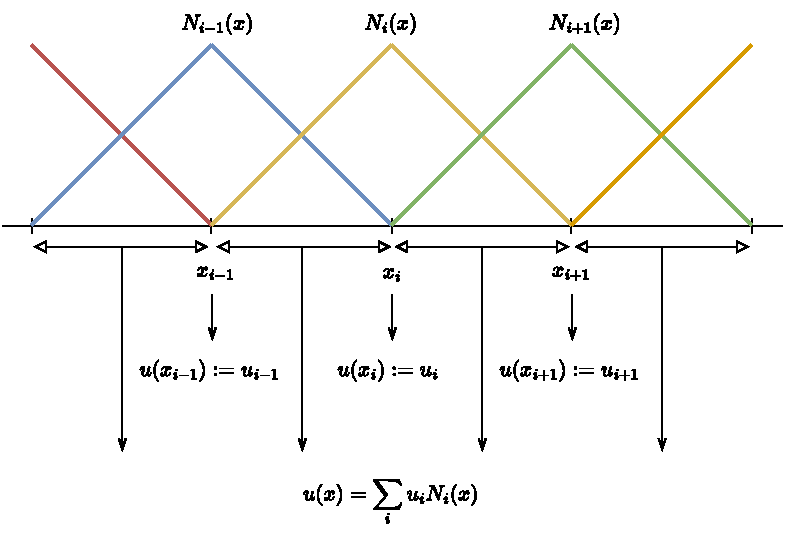
\includegraphics[trim={0 0 0 0},clip,width = 0.6\linewidth]{Figures/ShapeFunctions_1.drawio.pdf}    
    \caption{Treatment of points where the value of shape function is not defined correctly. }
    \label{fig:ShFDiscont}
\end{figure}


\section{Miscellaneous}

\Rq{In the mixed formulation, prescribing Neumann boundary conditions would be the same as imposing "Dirichlet boundary conditions" on the derivative field. It each space (primal and dual) the boundary conditions would be strictly prescribed, only the link between the primal and dual quantity would be weakly constrained through the loss.}

\Rq{Could have a hybrid training using both intergaral and mixed formulation ? To have a indicator of error on the integral versino aswell ?}
 
% \begin{figure}
%     \centering
%     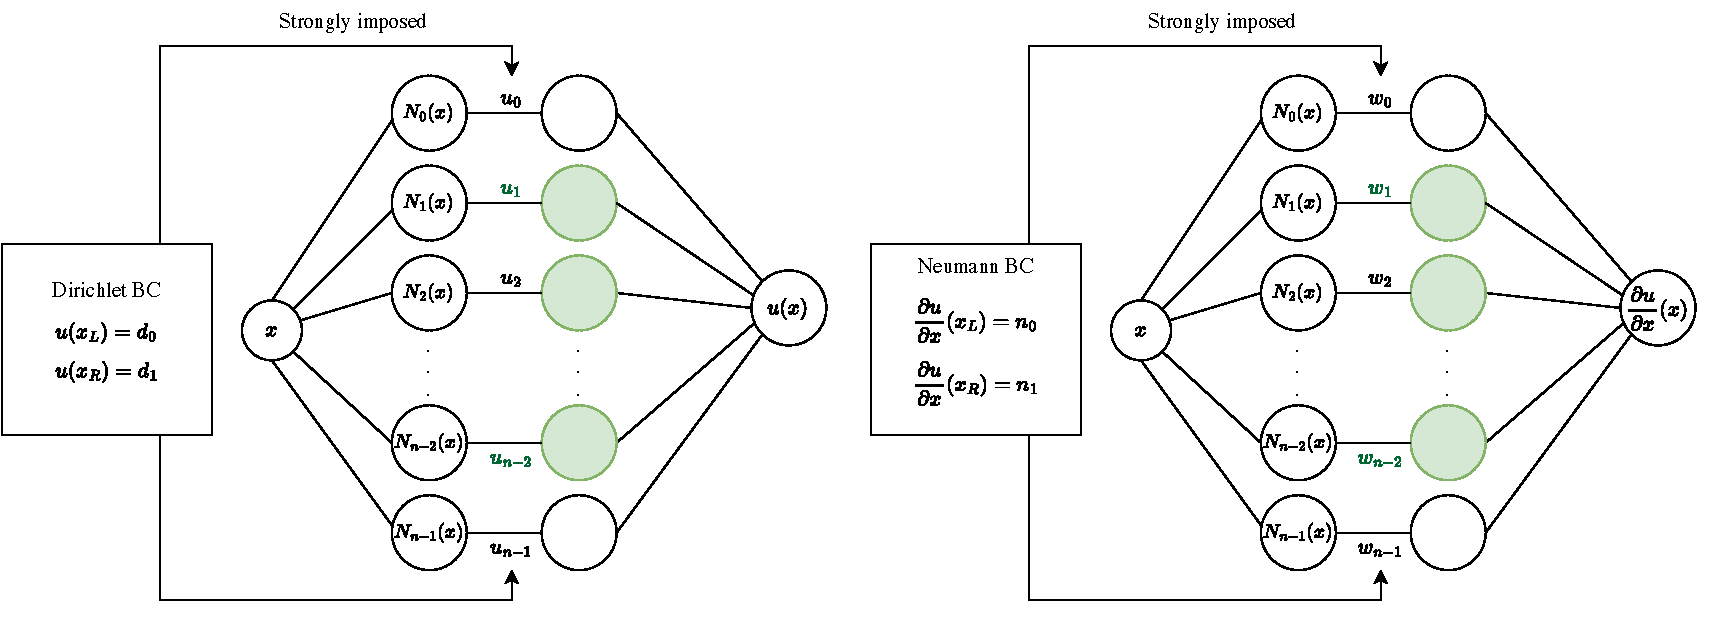
\includegraphics[trim={0 0 0 0},clip,width = 0.95\linewidth]{Figures/BC.drawio.pdf}    
%     \caption{Strong imposition of Dirichlet and Neumann boundary conditions in the associated NN.  }
%     \label{fig:ShFDiscont}
% \end{figure}

\begin{figure}
    \centering
    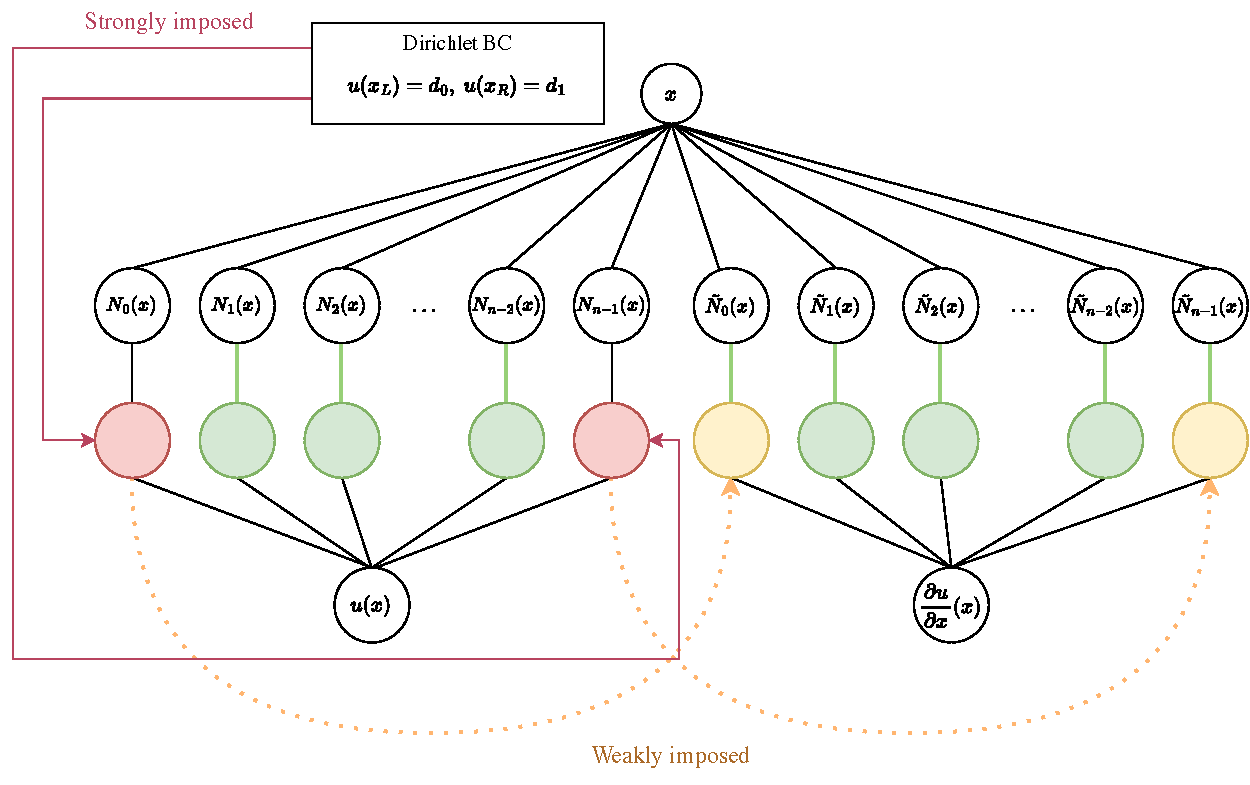
\includegraphics[trim={0 0 0 0},clip,width = 0.9\linewidth]{Figures/BC_1.drawio.pdf}    
    \caption{Neural network representation of mixed formulation for problem with Dirichlet boundary conditions. The boundary conditions are strictly prescribed for the NN providing the prediction of displacement $u$ and weakly (through loss function) for the NN providing the prediction of derivative of displacement $\frac{\partial u}{\partial x}$.   }
    \label{fig:BCsMixed}
\end{figure}


\section{Neumann boundary conditions}
\label{sec:NeumannMixed}
With the mixed formulation an important question concern the way boundary conditions are prescribed.

They can be seen as Dirichlet boundary conditions on the dual field, \emph{i.e.} constraints in the interpolation. A difficulty may arise when we want to implement relation constraints between different components. Indeed, in such a case the components are still free to evolve but under a given constraint.

Such a constraint can then be prescribed before evaluating the NN within the training loop so that it would be updated as the stress nodal quantities evolve as illustrated in \cref{alg:NeumannBCs}.



\RestyleAlgo{ruled}

%% This is needed if you want to add comments in
%% your algorithm with \Comment
\SetKwComment{Comment}{/* }{ */}
\SetEndCharOfAlgoLine{}
\begin{algorithm}[hbtp!]
	\caption{Prescribing Neumann boundary conditions during training}\label{alg:NeumannBCs}
	\textbf{Inputs: } \code{model\_stress}, \code{model\_disp}, \code{\{$\sigma_i$\}}, \code{\{$u_i$\}} \textcolor{GreenLMS}{\Comment*[r]{Two models and corresponding nodal quantities}}
	
	\While(\textcolor{GreenLMS}{\Comment*[r]{\hspace{-5pt}Training loop \hspace{-6pt}}}){Training}{
		Compute the $\vect{n}\text{ on }\partial \Omega$ \textcolor{GreenLMS}{\Comment*[r]{ Update the normal vectors on the BCs}}
		
		 \code{\{$\sigma_i$\}} $ = f$( \code{\{$\sigma_i$\}}, \code{\{$u_i$\}}, $\vect{n}$)  \textcolor{GreenLMS}{\Comment*[r]{ Boundary conditions constraints}}
		 
		 $\sigm \left(\vect{x} \right) = $  \code{model\_stress}$\left(\vect{x} \right)$ \textcolor{GreenLMS}{\Comment*[r]{ Stress evaluation}}
		 
		 $\vect{u} \left(\vect{x} \right) = $  \code{model\_disp}$\left(\vect{x} \right)$    \textcolor{GreenLMS}{\Comment*[r]{ Displacement evaluation}}
		 
		 $\mathcal{L} = \mathcal{L}\left(\sigm \left(\vect{x} \right) , \vect{u} \left(\vect{x} \right)  \right)$  \textcolor{GreenLMS}{\Comment*[r]{ Loss evaluation}}

		\code{optimiser.step}  \textcolor{GreenLMS}{\Comment*[r]{ Update the models}}

	}
\end{algorithm}
\newpage
\Rqs{The evlaluation of the stress is then done using nodale stress values in the \code{model\_stress} that are consistant with the boundary conditions.}{Such an implementation would also easily allow dealing with changing normal during training for large strains for instance.}

\textbf{\textcolor{accentcolor}{Question:}} The stress state is not fully defined by the Neumann boundary condition, \emph{i.e.} part of it comes from the admissibility and constitutive relation which is only verified at convergence. Prescribing in hard the remaining stress component from the displacement might help. 

\textbf{\textcolor{accentcolor}{Idea:}} give all our knowledge to the NN instead of learning what we already know. 

\textbf{\textcolor{accentcolor}{Question:}} In this idea, should we prescribe all nodal stress tensors except from where Neumann BCs are set ?
% \chapter[Transfer learning ++]{Transfer learning ++}
\label{chap:Transfer_learning}
\begin{chapabstract}
    This chapter highlights the superior capacities of transfer learning of the HiDeNN framework.
\end{chapabstract}

\minitoc

\section{Leveraging pre-trained model}

Because the architecture of HiDeNN is fully interpretable, the initialisation of the weights for a new (refined for instance) architecture can be done by using a previously trained architecture ( coarser one for instance).

\Rq{This is true for a new architecture with 
\begin{itemize}
    \item A refined space mesh
    \item A refined parametric mesh
    \item A different number of parameters
    \item A different number of modes
\end{itemize}}

\subsection{Training a finer space mesh}

When a new node $\ell$ is added at coordinate $\vect{x}_{\ell}$, the nodal value (the weights of the solution layer) can be initialised using the interpolation of the previously trained network as
\begin{equation}
    u_{\ell} = \vect{u}\left(\vect{x}_{\ell}\right).
\end{equation}

For a completely different mesh (refined) we can easily evaluate the coarse model on fine mesh and use the solution as initial nodal value for the fine HiDeNN. Here the finer model consist in a refined space mesh; the parametric mesh remains exactly the same.

A space refinement from $n_p = 20$ to $n_p = 60$ is investigated.
Illustrations of different initialisation strategies are given in \cref{fig:TransferSpace} where 
\begin{equation}
    \Xi = \frac{\Vert\overline{ \vect{u}_{NN}-\vect{u}_{\text{exact}}}\Vert}{\Vert\overline{ \vect{u}_{\text{exact}}}\Vert}.
\end{equation}

$\overline{\square}$ is the average of the quantity $\square$ over the samples of $E$.

\begin{figure}
    \begin{subfigure}[t]{0.5\linewidth}
        \centering
        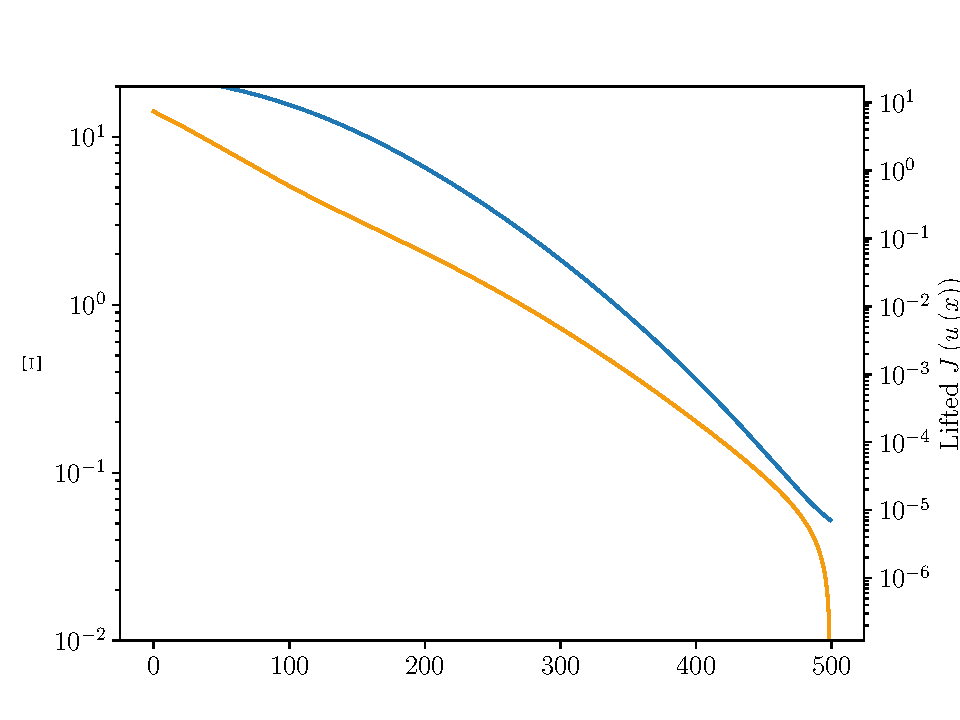
\includegraphics[width=\linewidth]{Figures/ParaError_NoInit.pdf}
        \caption{No initialisation}
    \end{subfigure}
    \begin{subfigure}[t]{0.5\linewidth}
        \centering
        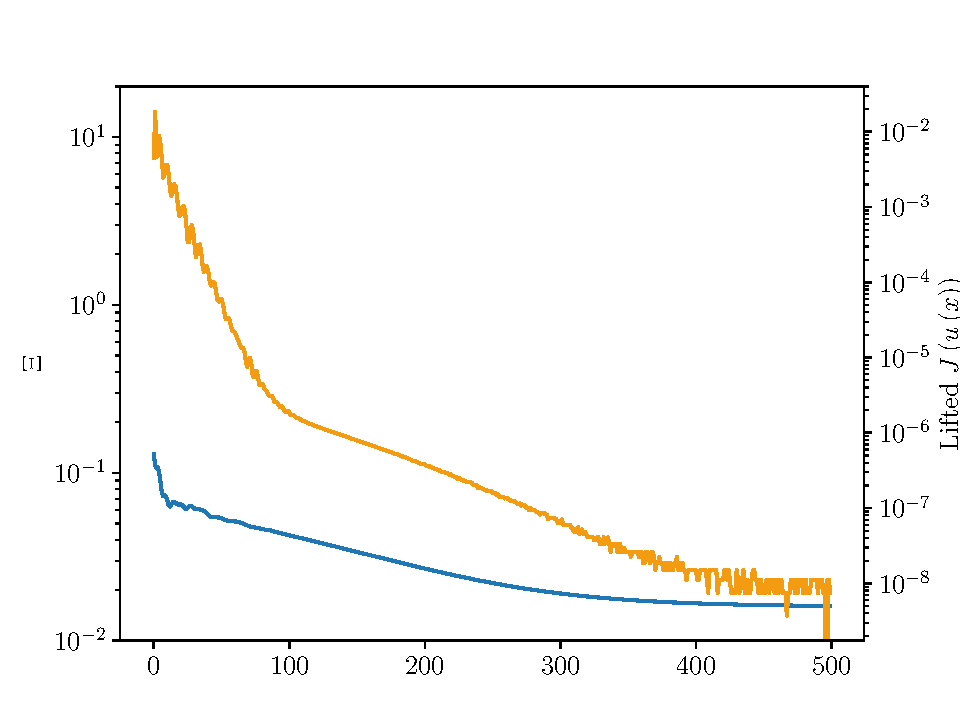
\includegraphics[width=\linewidth]{Figures/ParaError_full_initialised.pdf}
        \caption{Space and parameter modes initialised}
    \end{subfigure}
    \begin{subfigure}[t]{0.5\linewidth}
        \centering
        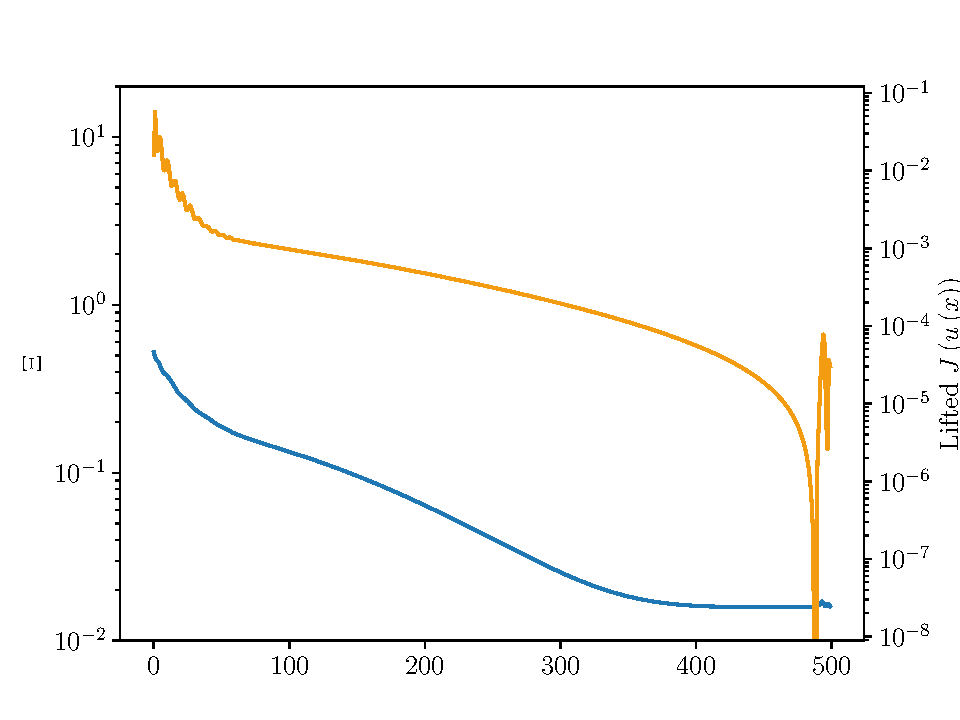
\includegraphics[width=\linewidth]{Figures/ParaError_space_initialised.pdf}
        \caption{Space mode initialised}
    \end{subfigure}
    \begin{subfigure}[t]{0.5\linewidth}
        \centering
        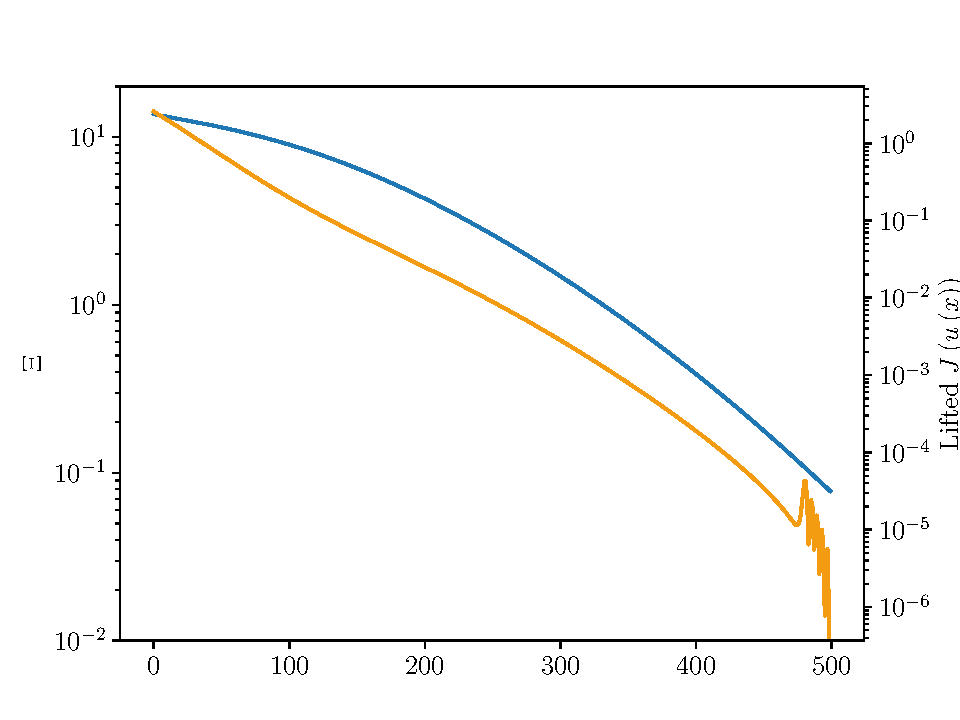
\includegraphics[width=\linewidth]{Figures/ParaError_para_initialised.pdf}
        \caption{Parameter mode initialised}
    \end{subfigure}
        \caption{Loss and $\mathcal{L}^2$ error}
    \label{fig:TransferSpace}
\end{figure}

An illustration of the use of pretrained coarse modes to quickly get a fine mode is illustrated in \cref{fig:InitialisationModes_Coarse}.

\begin{figure}
    \begin{subfigure}[t]{0.5\linewidth}
        \centering
        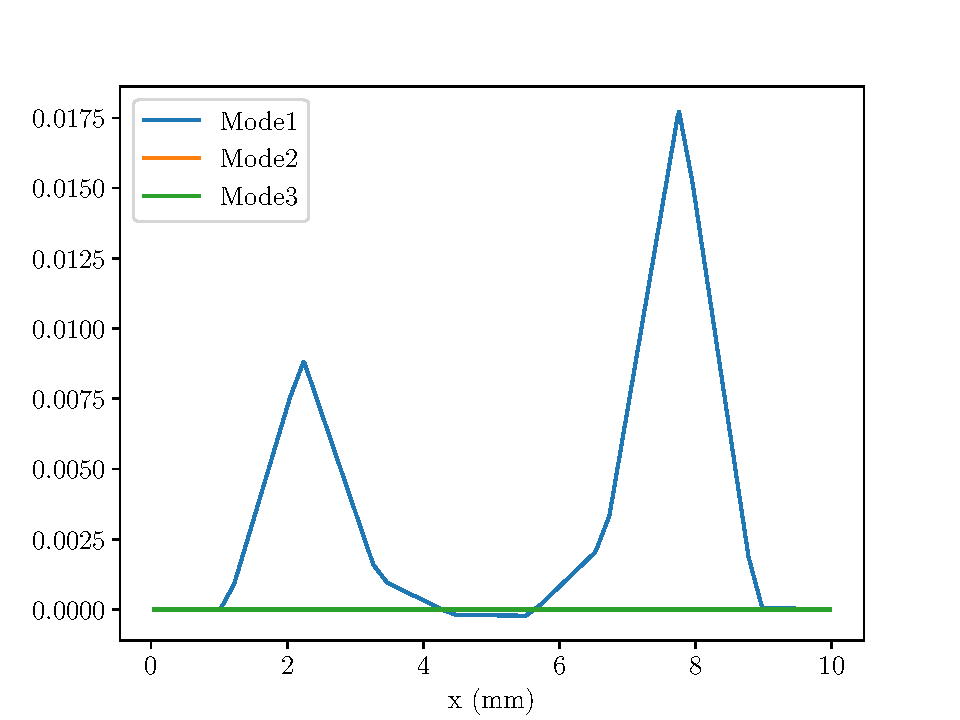
\includegraphics[width=\linewidth]{Figures/Pre_trained_Space_modes3.pdf}
        \caption{Pre-trained space mode initialisation on $1$ mode \& $n_p=10$}
    \end{subfigure}
    \begin{subfigure}[t]{0.5\linewidth}
        \centering
        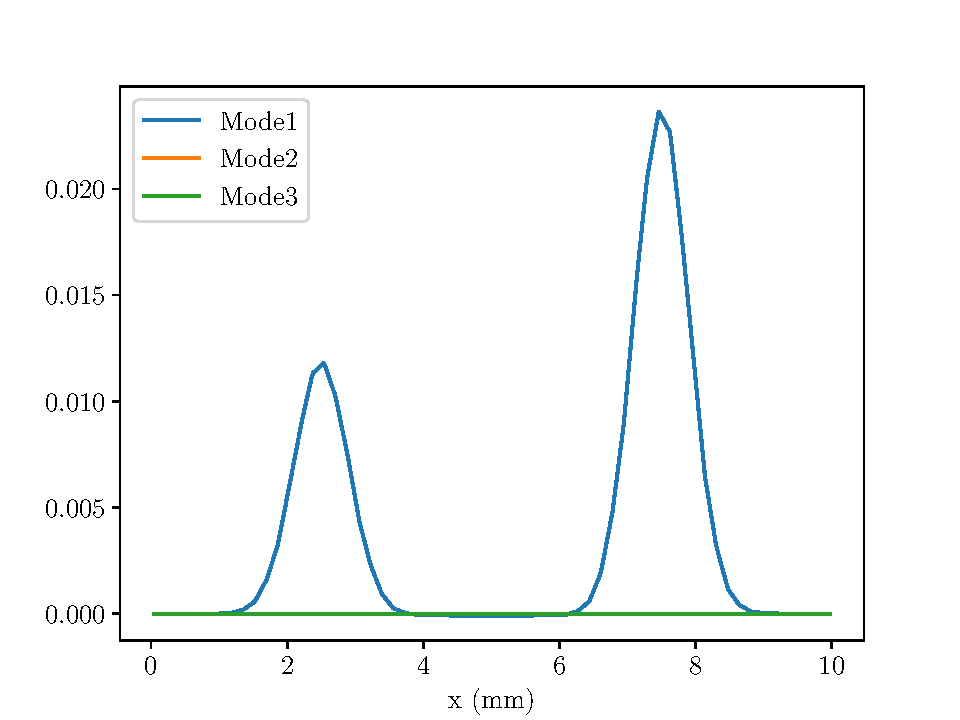
\includegraphics[width=\linewidth]{Figures/Trained_Space_modes3.pdf}
        \caption{Trained space modes}
    \end{subfigure}
    \caption{Modes initialisation (from 1 mode \& $n_p=10$ to $3$ modes \& $n_p=50$.}
    \label{fig:InitialisationModes_Coarse}
\end{figure}

\subsection{Link with literature}

\cite{giacoma_toward_2015} showed that using a coarser mesh to initialised the reduced-order basis can drastically decrease the number of required iterations to build a reduced-order model. Using the NN-PGD based on the hiDeNN framework, this idea can easily be used in the training strategy to start with coarser mesh and transfer the computed mesh onto the more refined mesh later in the training.
% \chapter[Notes to ourselves]{Notes to ourselves}
\label{chap:Note}
\begin{chapabstract}
    This chapter summarises our notes and remarks as we have progressed in our understanding of the subject.
\end{chapabstract}

\minitoc

\section{Implementation}
    Many of the elementary blocks described by \cite{zhang_hierarchical_2021} can be achieved using elementary tensor algebra (addition multiplication, etc.).
    \begin{itemize}
        \item Using \emph{perceptron} as the sole building block for all operations as done in \parencite{zhang_hierarchical_2021} leads to a generic implementation where the gradient is always well populated.
        \item Relying on \textsc{Pytorch} tensor operations lead to the same results but appears to be faster when available.
        \begin{itemize}
            \item When available, using \textsc{Pytorch} operations might be easier and, therefore, more efficient overall when implementing new features.
        \end{itemize}
    \end{itemize}

    \subsection{Saving Models}

    When the architecture is expected to change a lot saving the full model as opposed to solving the model state dictionaries makes it easier to reuse a previously saved model associated with an older architecture. 

    \section{Code}
    \subsection{Efficiency}
    \subsubsection{Module ensembling}
    The sub neural networks are stored in \code{ModuleList} object and are called through list comprehension.
    \code{ModuleList} should support slicing and list comprehension might be the reason why the implementation is so slow !! \href{https://github.com/pytorch/pytorch/issues/37718}{Discussion about this subject} Model ensembling shown \href{https://pytorch.org/functorch/stable/notebooks/ensembling.html}{here} is also promissing but it seems that \href{https://pytorch.org/functorch/stable/}{functorch} is depreciated and a \href{https://pytorch.org/docs/master/func.migrating.html}{migration} to \href{https://pytorch.org/docs/stable/func.html}{torch.func} is advised. Using the concatenation and vmap should allow getting rid of for loop or list comprehension.

    \subsubsection{Vectorisatoin at the Element scale}

    As I was unable to use module ensembling and \code{torch.vmap} on our implementation, I ended up re-writing the Element block so that it computes all elements in parallel in a vectorised fashion. Doing so means that there is a single \code{ElementModule} that inputs all the element indexes as oppose to having a library of all the elements of the mesh.

    \subsubsection{Comparison with classcial FEM solvers}
    \cite{park_convolution_2023} emphasise in their abstract that in order to get similar computational time with HiDeNN as we get with standard FEM solvers on CPU they have to use GPUs.
    \Rq{The comparison does not really make sens anymore as the hardware is different but that provide a good insight on order of magnitude of the computational time differences they are experiencing.}
\subsection{NeuROM}
 In the parametric context, the implementation can be made so that the constitutive blocks are very general and so that no changes are required in the interpolating architecture. The HiDeNN architecture is therefore written once for any kind (different number of parameters, different discretisation of the parameter spaces, and so on)  of problem. 

 However, the loss function is problem dependent, the implementation difficulty for a new problem therefore lies in writing the loss function in an appropriate and efficient manner.

\subsubsection{Training}

It seems that the \code{deep\_copy} of state dict is very slow, should monitor its impact and if needed think of a way to make it faster.


 \section{Ressources on Jean-Zay}
\label{sec:JZ}
 In order to get access to (free) ressources on Jean-Zay we need to provide

 \begin{itemize}
     \item Title
     \begin{itemize}
         \item Real-time simulation and individualisation of the human lung
     \end{itemize}
     \item Thematic (Note that no matter what we select we later have to specify whether or not we use AI)
     \begin{itemize}
         \item CT3 Biologie et santée
         \item CT6 Algorithmique, informatique et mathématiques 
         \item CT10 Inteligence artificielle et applications transversales de calcul 
     \end{itemize}
     \item Public summary of the project 
     \begin{itemize}
         \item This project aims to provide clinicians with diagnostic and prognostic tools based on mechanical simulation. Therefore, it is necessary to set up numerical tools that give access to mechanical quantities computed in real-time for each patient, i.e., to allow on-the-fly evaluation of the complex mechanical model for a new set of parameters. Therefore, The idea is to couple classical model-order reduction methods with machine learning capabilities to provide a fine-tuned solution to the highly non-linear mechanics problem in real-time. In order to achieve interpretability of the neural network parameters and to limit their number, this work is based on the HiDeNN framework, which proposes to constrain the interpolation offered by the neural network to interpolation by shape function similar to the interpolation of fields when using the finite element method. This framework also allows great flexibility in transfer learning between different models. When a model is refined, the information learned during training of a coarser model can be transferred to the refined model, allowing great efficiency in the model's design and limiting the wasteful use of resources.
         
A second way of making the method as efficient as possible is to use the tensor decomposition classically used in model-order reduction to avoid the curse of dimensionality, which means that the number of unknowns in a problem grows exponentially with the number of parameters.

The goal is to use this hybridisation between model-order reduction and machine leaning to make a complex lung model clinically usable by providing a virtual abacus of this model for a large number of parameters, i.e. by providing a parametric digital twin of the lung which would be numerically inexpensive.
     \end{itemize}
     \item Technical representative
     \begin{itemize}
         \item abdelfattah halim
     \end{itemize}
 \end{itemize}

\section{Optimizer}

The \code{Adagrad()} optimizer does not seem to add any improvement over standard adam method even in the case of parametric implementatin where the difference in the magintude of the compnent could have given the edged to adagrad method as different learning rate for each of the parameters would have made sense.


\section{Parametric efficiency}

\subsection{Efficiency findings}
When the number of parameters increases the cost drastically increases and I do not know why. 


\subsection{Different implementation strategies}
Basically the parameters and the modes are handled as a list of Modules (functions) that are indexed by the mode number and the parameter number. Each function within the list is well vectorised.


\paragraph{The first non optimal idea is to use for loops}

Two nested loops to iterate through the functions stored in \code{self.Para\_modes}.
\RestyleAlgo{ruled}

%% This is needed if you want to add comments in
%% your algorithm with \Comment
\SetKwComment{Comment}{/* }{ */}
\SetEndCharOfAlgoLine{}
\begin{algorithm}[hbtp!]
	\caption{Parameter modes evaluation}\label{alg:two}
	\textbf{Inputs: } \code{Para\_mode\_Lists}, \code{mu} \textcolor{GreenLMS}{\Comment*[r]{List of Modules and parameters samples mu}}
	
	\For(\textcolor{GreenLMS}{\Comment*[r]{\hspace{-5pt}Loop over the modes\hspace{-6pt}}}){$k \in \llbracket 1,m \rrbracket$}{

	\For(\textcolor{GreenLMS}{\Comment*[r]{\hspace{-5pt}Loop over the parameters\hspace{-6pt}}}){$k \in \llbracket 1,\beta \rrbracket$}{
            \code{Para\_mode\_List[mode][l] = self.Para\_modes[mode][l](mu[l]) 
            }
    }
    }
\end{algorithm}

\paragraph{List comprehension}

The for loops can easily be converted to list comprehension.

\begin{algorithm}[hbtp!]
	\caption{Parameter modes evaluation}\label{alg:two}
	\textbf{Inputs: } \code{Para\_mode\_Lists}, \code{mu} \textcolor{GreenLMS}{\Comment*[r]{List of Modules and parameters samples mu}}
	
\code{Para\_mode\_Lists = [[self.Para\_modes[mode][p](mu[p])} 
\code{for p in range(self.n\_para)]for mode in range(self.n\_modes)]}
\end{algorithm}

No speed-up is observed. The \code{ModuleList} offers the same syntax as python lists but the implementation might differ.

\paragraph{Vectorisation over the indexes} Because the output of each functions in \code{ModuleList} are independent from one-another it would be perfectly possible to run their evaluation in parallel. To that aim several vectorisation implementation where tried with little to no success.

\begin{itemize}
    \item Slicing does not work on Module or function lists
    \item There's no way to vmap directly over an array of functions \href{https://github.com/google/jax/issues/673}{see this topic}
    \item There is a workaround using switch (not implemented in \textsc{pytorch} yet but works with jax)
\end{itemize}

I tried the workaround proposed \href{https://github.com/google/jax/issues/673}{here} using jax to compare the speed up results and.... it was way worse (10x slower than using for loops).

I tried \code{jax.jit} over the vmaped function and it was even worse (100x slower than using for loops)

\Rq{Those findings might be linked to early versions of jax not being well optimised for M2 chips yet}


\paragraph{Results:}
On a simpler example the evaluation of the above mentioned methods was tried and yield the conclusion that on our hardware the list comprehension might be the best way to go.
\begin{verbatim}
**** Example 1 ****
For loop:               t = 1.180887222290039ms
List comprehension:     t = 1.0099411010742188ms
vmap:                   t = 100.78692436218262ms
\end{verbatim}


\paragraph{Investigation on why it is so slow}

with one parameter the complexity seems to be O(m) which sounds reasonable.

If I fix $m=1$ and go from $1$ parameter to $2$, the running time per epoch increases by a factor $5$.

\Rqs{It might be due to the loss implementation that somehow brings back the curse of dimensionality. It does not seem easy to remove the full tensors field evaluation to compute the integral due to the square of the gradient $$\left( \frac{\partial u}{\partial x} \right)^2 = \left( \sum\limits_{i=1}^m \textcolor{BleuLMS!70}{\frac{\mathrm{d}\overline{\vect{u}}_i(\vect{x}) }{\mathrm{d}x}} ~\textcolor{LGreenLMS}{\prod_{j=1}^{\beta}\lambda_i^j(\mu^j)} \right)^2$$}{Try to rely on  the orthogonality of the space modes (which we do not have currently but could be post-processed with GS or constrained )}


\Rq{It could be interesting to have fine batches in the x direction and have mini-natches for the parameters to remove the curese of dimensionality somehow or lessen it.}
\chapter[Conferences abstracts]{Conferences abstracts}
\label{chap:conf}
\begin{chapabstract}
    This chapter regroups all abstracts written for conferences
\end{chapabstract}

\minitoc

\section{VPH: Virtual physiological human}
Data-Driven Simulation Technologies for Clinical Decision Making
\begin{itemize}
    \item 4-6 September 2024
    \item University of Stuttgart
\end{itemize}

\subsection{Parametric paper}
\paragraph{Hybridising standard reduced-order modelling methods with interpretable sparse neural networks for real-time patient specific lung simulations}

Stress fields possibly play a crucial role in the development of pulmonary fibrosis. This work, aims to provide clinicians with diagnostic and prognostic tools based on mechanical simulation. Personalisation of these tools is critical for clinical pertinence, thus requiring numerical techniques for real-time estimation of patient-specific mechanical parameters.

This work proposes hybridising classical model-order reduction methods with machine learning capabilities to provide a fine-tuned real-time solution to the highly non-linear mechanics problem. 

Analogous to techniques like the Proper Generalised Decomposition (PGD) or the Higher Order Singular Value Decomposition (HOSVD), the parametric mechanical field is represented through tensor decomposition, effectively mitigating the curse of dimensionality associated with high-dimensional parameters. Each mode of the tensor decomposition is given by the output of a sparse neural network within the HiDeNN framework, constraining the weights and biases to emulate classical shape functions used in Finite Element Method.

This hybridisation preserves interpretability while affording greater flexibility than standard model-order reduction methods. For instance, it allows for employing diverse meshes for individual modes in the tensor decomposition, with the added capability of mesh evolution during the training stage. Moreover, the model's architecture results directly from the number of nodes and the order of elements used for interpolation, thus eliminating the need for arbitrariness in its choice.

In this framework, the training stage amounts to solving the minimisation problem classically encountered with classical model reduction methods, but the automatic differentiation tools naturally available in the neural network framework allow greater flexibility in solving this minimisation problem when a linearisation of the problem is not straightforward. 
Finally, this framework allows for transfer learning between different models with different architectures, leading to high efficiency in the model's design and limiting the wasteful use of resources.

\subsection{Mixed formulation}
\paragraph{Bridging Micro to Macro in Pulmonary Mechanics: Interpretable Neural Networks for Surrogate Modelling}
Idiopathic Pulmonary Fibrosis (IPF) is a disease characterized by the progressive formation of scar tissue in the lungs, leading to locally increased tissue stiffness and impaired respiratory function. Despite its significant impact on patient health, IPF remains poorly understood and poorly diagnosed. Our focus on IPF is motivated by the complex impact the fibrosis has not only on the lung tissue structure but also on the lung kinematics, and mechanics. The coupling between the disease progress and mechanical environment, as well as the multiscale nature of the disease, calls for a multiscale modeling approach to connect phenomena arising on various spatial scales. In order to integrate the existing micromechanical and organ-level models, the micro-model needs to undergo reduction. In our work, we propose to address this challenge by using a machine learning-based surrogate modeling framework.

In the presented framework, we use structured neural networks designed to be able to produce standard FEM shape functions. Similarly, to classical Physics-informed neural networks, this framework also has the capability to incorporate mechanistic knowledge through appropriate definition of the loss function. Due to the specific structure of the neural network, the number of trained parameters is significantly lower compared to a fully connected neural network and the individual weights and biases have a clear interpretation. In addition to higher reliability, the interpretability also allows us to strongly impose Dirichlet boundary conditions and thus avoid some of the changes caused by including additional terms in the loss function.

In this contribution, we present the capabilities of the model on several 1D and 2D test cases. The architecture of the neural network is defined by the discretization of the domain on which the governing equations are solved. There are however other choices, that effect the results, including the definition of the loss function and selection of optimizer and training strategy. We discuss the benefits and limitation of the tested variants and show how they affect the results obtained by the model.

\clearpage{\thispagestyle{empty}\cleardoublepage}

\part{Codes}
\chapter[Code instructions]{Code instructions}

\begin{chapabstract}
    A Python implementation of the above-mentioned frameworks is available on the INRIA \href{https://gitlab.inria.fr/aldabyse/hidenn_1d}{Gitlab}.
\end{chapabstract}

\minitoc
\section{Code presentation}

\begin{itemize}
	\item \textcolor{accentcolor}{\textbf{Name:}} NeuROM: Sparse Interpretable Neural ROM
	\begin{itemize}
		\item Combines Neural + ROM
		\item Sounds like Neuron
		\item Sounds like New ROM
	\end{itemize}
\end{itemize}
\section{Implementation of a HiDeNN for a 1D Bar}

The objective of this code is to provide an implementation of a HiDeNN. The layer's input is the coordinate $\vect{x}$ where the output is evaluated. In this case, the output of the network is the displacement $\vect{u}\left(\vect{x}\right)$

The first hidden layers play the role of linear shape functions by applying constraints on the weights and bias of sub-networks composing the first layers. The last hidden layer called the interpolation layer in the remainder of the document, utilises the output of the shape functions to interpolate the output. Training the weights of that last hidden layer is the same as solving a FEM problem on a fixed mesh. The weights of the interpolation layer directly correspond to the nodal values associated with each shape function. Therefore, prescribing Dirichlet boundary conditions is straightforward by freezing the weights associated with the prescribed values of fixed DoFs.

\subsection{Architecture of the NN}


\begin{itemize}
    \item Linear left and right classes that are the two elementary blocks to create a linear 1D shape function
   \item Shape class that are based on the two aforementioned building blocks and, given an index, build the shape function associated with that index i
   \item MeshNN class that, given geometric parameters, "assemble" the shape functions accordingly
    \begin{itemize}
        \item \code{model = MeshNN(np,L)}
        \item np \& L being the number of DoFs and the length of the bar, respectively
   \end{itemize}
   \item The Dirichlet boundary conditions (BCs) are set by calling
   \begin{itemize}
        \item \code{model.setBCs(u\_0,u\_L)} 
        \item with $u_0$ and $u_L$ being the prescribed displacement at $x=0$ and $x=L$ respectively
        \end{itemize}
\end{itemize}

\subsection{Training the NN }

The Volumic forces are accounted for in the loss function through the right-hand side (RHS) function, and the loss function is the potential energy.

The trainable parameters can be changed on the fly. 
\begin{itemize}
    \item \code{model.Freeze\_Mesh()} Freezes the mesh so that only the nodal values are trained
    \item \code{model.UnFreeze\_Mesh()} Unfreezes the mesh so that the coordinates values can be trained
    \item \code{model.Freeze\_FEM()} Freezes the nodal values so that only the coordinates are trained
    \item \code{model.UnFreeze\_FEM()} Unfreezes the nodal so that the FEM problem can be solved
\end{itemize}


\section{Parser}

As usually done in a Finite element (FE) framework, interpolating the quantities of interest in the spatial domain is achieved using shape functions associated with a mesh.
\Rq{The difference being that the input and output are ``post-processed'' in the sense that the underlying mesh is invisible to the user. Another difference is that the mesh used to initialise the HiDeNN is not fixed and can be adapted throughout the training process. Only the external nodes of the mesh, describing the structure's geometry, are fixed to conserve the structural shape of the strudied object.}

In order to convert information from the mesh to the HiDeNN architecture, a parser is required.

\subsection{Mesh format}
This parser relies on the \code{.msh} format exported in the \code{Mesh.MshFileVersion = 2.2}.


\section{Implementations}

\Rq{Note that the assembly matrix (just as the assembled stiffness matrix in a FE code) is not created through for loops but in a vectorised way so as to minimise overhead costs.}


The shape functions in 1D are sorted so that the in an element the node associated to the left part of a shape function is above the node associated to the right part of the shape function. 
Note that this lead to the two part of the shape functions not to be adjacent in the output intermediate layer. as illustrated in \cref{fig:SortingSF}.

\begin{figure}
    \centering
    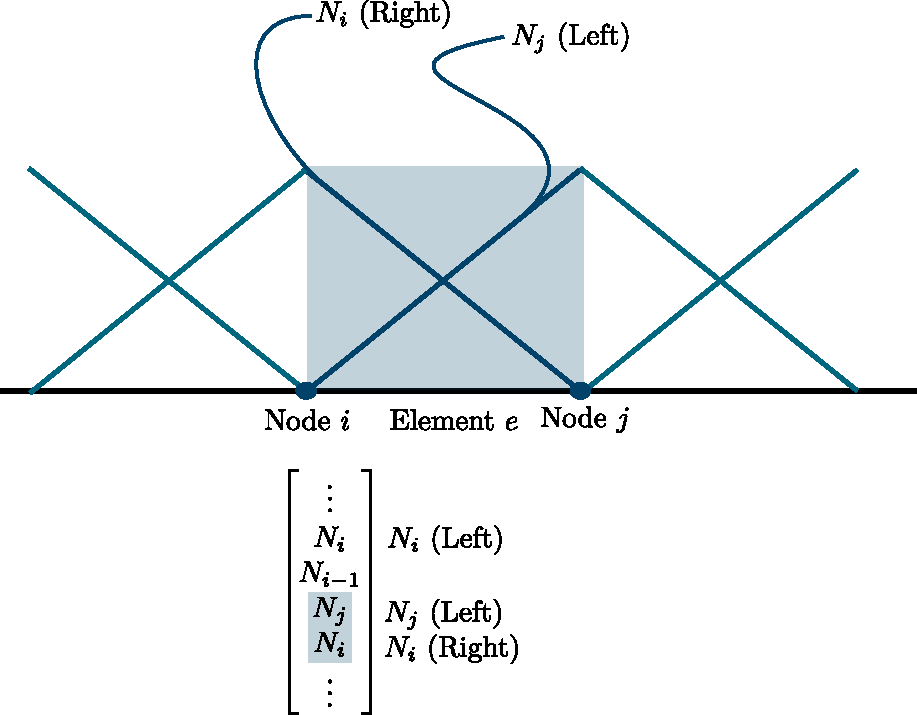
\includegraphics[width = 0.7\linewidth]{Figures/SortingOfShapeFunctions.pdf}
    \caption{Sorting of the shape functions in each element}
    \label{fig:SortingSF}
\end{figure}
% \chapter[Technical TODOs]{Technical TODOs}

\begin{chapabstract}
    A Python implementation of the above-mentioned frameworks is available on the INRIA \href{https://gitlab.inria.fr/aldabyse/hidenn_1d}{Gitlab}.
\end{chapabstract}

\minitoc

\section{Reusing previous training}

One significant advantages of HiDeNN architecture is its ability to benefit from previous training when being refined thanks to its interpretable nature. 

In order to benefit from such a propriety, an efficient model saving and model loading strategy needs to be set up. Indeed the saving and loading on-the-shelf functions of pytorch do not allow for changes in the architecture so a way to utilise such functions while still allowing the architecture to evolve is required.

\begin{itemize}
    \item Save sub independent neural networks and load them individually
    \item iterate through all parameters manually 
    \item Load model on same architecture and then modify it
\end{itemize}

On key element is that because we know what the parameters mean we can also initialise the new parameters wisely. For instance when a new node $\ell$ is add at coordinate $\vect{x}_{\ell}$, the nodal value (the weights of the solution layer) can be initialised using the interpolation of the previously trained network as
\begin{equation}
    u_{\ell} = \vect{u}\left(\vect{x}_{\ell}\right).
\end{equation}

\paragraph{What could be done:} 
\begin{itemize}
    \item Get a finer mesh
    \item Save untrained fine model
    \item Load a coarser pre-trained model
    \begin{itemize}
        \item Get a parser to read the difference in both architecture
        \item \code{model = torch.load(`Model')}
        \item \code{model.keys()} to get the entries 
        \item \code{model[`Space\_modes.0.NodalValues\_uu']} to get the number of nodal values for instance and their values
    \end{itemize}
    \item Evaluate the coarse model on fine mesh
    \item Update the \code{model state} dictionary for the new fine architecture using the evaluated values (leave the new values at their initial state)
    \item Load that dictionary on the fine model
\end{itemize}

\Rq{Once this works we could use that propriety during training and use a coarse mesh for the first training iterations and use the solution of that pre-training as a ``macro solution'' for the finer simulation thus decreasing the number of ``costly'' training iterations while still getting a fine solution.}

That works, 
\begin{itemize}
    \item Decide what to do with training (freeze part of the pre-trained network to get out of local minimum?)
\end{itemize}



% % Appendices
% \thesisappendix

% \input{chapters/appendices/my_first_appendix.tex}
% \clearpage\null

%%% Backmatter
\backmatter
% Display the bibliography
\defbibheading{bibintoc}{\addcontentsline{toc}{part}{\bibname}}
\chapter*{\bibname}
\printbibliography[heading=bibintoc]

\end{document}